\chapter{Sviluppo del progetto}
In questa sezione verrà illustrato lo sviluppo del progetto, seguendo le varie fasi che hanno portato alla realizzazione del modello
per la generazione condizionata di immagini con difetti, partendo da una descrizione generale della pipeline di addestramento
e delle sue componenti, per poi passare alla descrizione delle varie fasi di sviluppo, con particolare attenzione alla fase di
preparazione dei dati e alla fase di addestramento del modello. Verrà inoltre discussa la valutazione del modello mediante FID. 

\section{Definizione della pipeline di addestramento}
\begin{comment}

    Punti principali da affrontare:
        - Introduzione alla pipeline di addestramento:
            Stabilità e qualità nell'addestramento del modello.

        - Obiettivi della pipeline di addestramento:
            Generazione realistica di immagini con difetti.

        - Descrizione delle componenti della pipeline:
            Dataloader, trainer e script di evaluation inclusi.

\end{comment}
Questa pipeline di addestramento per la generazione dei difetti è stata principalmente ispirata dalla pipeline di LaMa, alla quale però
è stato necessario apportare diverse modifiche per poter ottenere il risultato desiderato.
Il task effettuato da LaMa infatti si basa sulla ricostruzione di parte dell'immagine originale, alla quale viene cancellata una certa porzione prima di passarla
al generatore, mentre il task che si vuole effettuare in questo progetto è quello di modificare l'immagine aggiungendo delle caratteristiche
appartenenti ad una o più distribuzioni. Come visto precedentemente, il modello di LaMa è stato addestrato
prendendo in input un'immagine con una certa porzione rimossa, concatenata con una maschera che indica la posizione della porzione rimossa,
alla quale eventualmente viene aggiunto del rumore gaussiano per favorire la generalizzazione del modello e una maggiore variabilità dell'output.
Per quanto riguarda COIGAN il condizionamento dell'output avviene nella medesima maniera, ovvero concatenando delle maschere all'immagine,
diversamente da LaMa le aree corrispondenti alle maschere e dunque alla porzione di immagine sulla quale vanno applicati i difetti non viene rimossa, 
in quanto quest'ultima contiene delle informazioni utili per la generazione di un output più coerente con l'immagine originale.\\
Di seguito è rappresentato un'esempio di input, con i primi tre canali del tensore di ingresso rappresentanti l'immagine base,
mentre i successivi 4 canali rappresentano le maschere per il condizionamento dell'output.\\

    \begin{figure}[H]
        \centering
        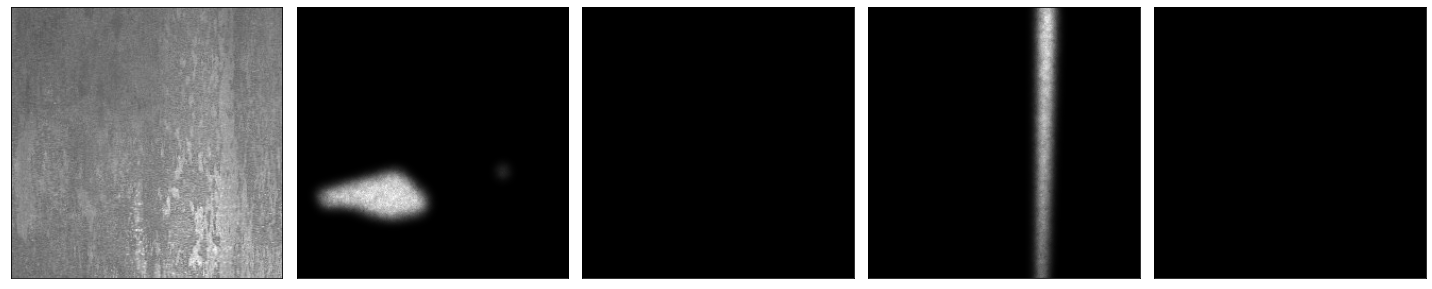
\includegraphics[width=0.9\textwidth]{imgs/Coigan/G_input.png}
        \caption{Figura che illustra un esempio di input di COIGAN, il quale è un tensore di 7 canali, in questo caso con un'immagine RGB e 4 canali
        per le maschere che effettuano il condizionamento della generazione dei difetti.} 
        \label{fig:Coigan input}
    \end{figure}

Nella Pipeline di LaMa come visto nella sezione \ref{sec:lama}, ci sono 3 loss principali, esclusa la regolarizzazione, le quali sono:
la loss L1, la \textit{Adversarial loss} e la \textit{Perceptual loss}. La loss L1 è una componente della loss che spinge il generatore verso
il centro della distribuzione dei dati, la quale anche se come illustrato da Goodfellow può portare a risultati non ottimali, per quanto visto
nella pubblicazione di Pix2Pix, se utilizzata con il giusto peso in congiunzione con l'\textit{Adversarial loss} sembra migliorare i risultati generali.
La \textit{Adversarial loss} è la componente principale della loss, che spinge il generatore a generare immagini che abbiano delle caratteristiche
appartenenti alla distribuzione del \textit{training set}. In fine la \textit{Perceptual loss} è una componente che spinge
il generatore a completare l'immagine con delle caratteristiche che siano coerenti con quelle della parte rimossa dell'immagine originale, senza bisogno di effettuare
un match perfetto, quest'ultima applicata con le \textit{features} di un modello preaddestrato e attraverso quelle estratte dal discriminatore.

    \begin{figure}[H]
        \centering
        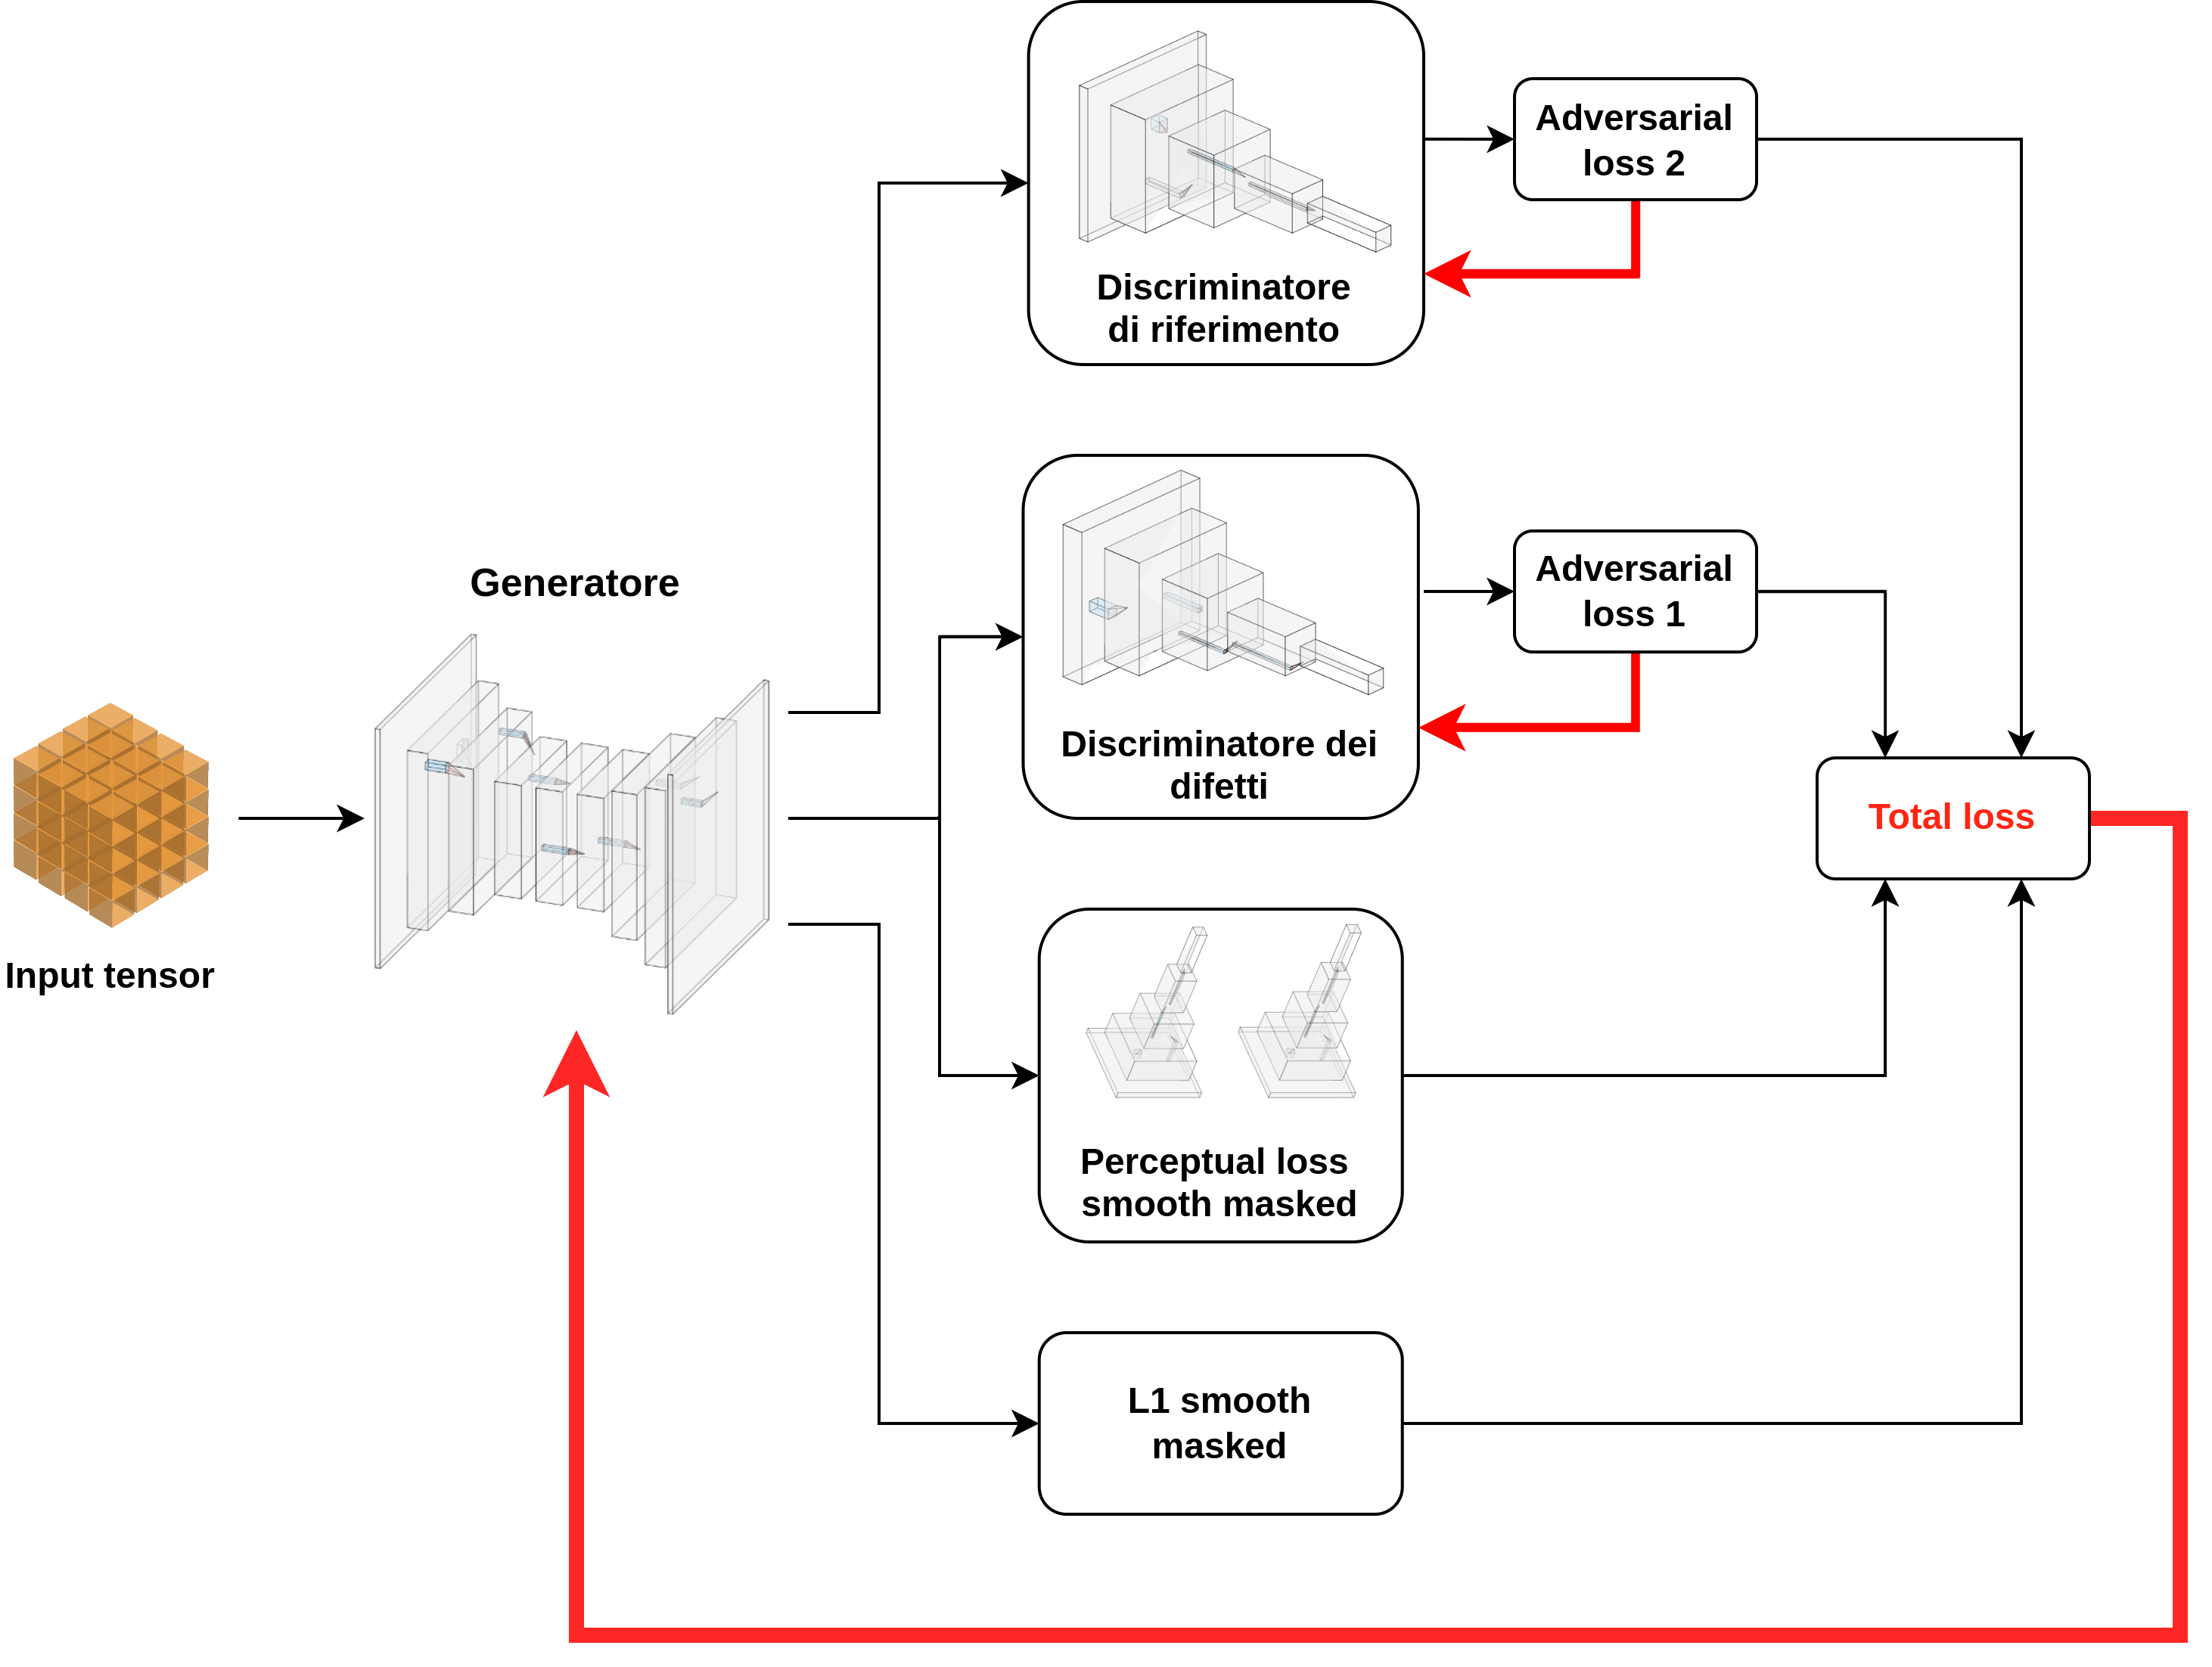
\includegraphics[width=0.9\textwidth]{imgs/Coigan/General pipeline schema.png}
        \caption{Figura che illustra in maniera riassuntiva le componenti principali della pipeline di addestramento di COIGAN.
        le frecce rappresentano la propagazione dei vari tensori, mentre le linee rosse indicano la propagazione dei gradienti delle loss.} 
        \label{fig:pipeline_di_addestramento}
    \end{figure}

Per quanto riguarda COIGAN, le modifiche principali che sono state apportate sono relative a come sono state utilizzate le adversarial loss, e all'introduzione
di una \textit{smooth mask} per pesare la loss L1 e la \textit{Perceptual loss}. In oltre ci sono delle modifiche sostanziali nella preparazione dei dati,
i quali in questo caso non vengono utilizzati direttamente come input del generatore, applicando semplicemente una maschera per rimuovere una certa porzione.
Nella Figura \ref{fig:pipeline_di_addestramento} è riassunta la pipeline di addestramento, per la quale in seguito verranno approfondititi i vari componenti.\\

\section{Preparazione dei dati per la pipeline}
\begin{comment}
    In questa sezione discuto principalmente del dataset e di come questo viene preparato per l'addestramento del modello.
    
    sottosezioni:
    1 - formato originale del dataset
    2 - conversione del dataset nel formato jsonl
    3 - fair split del dataset
    4 - creazione del dataset degli oggetti
    5 - creazione del dataset di immagini base
    6 - creazione dei dataset utilizzati come riferimento

\end{comment}

In questa sezione verrà illustrato come è stato preparato il dataset per la pipeline di addestramento, partendo dal dataset
Severstal steel defect detection dataset, nel suo formato originale, per poi passare alla conversione del dataset nel formato \textit{line json},
utilizzato poi anche dal dataloader della training pipeline.
Verrà illustrato come è stato effettuato un \textit{fair split} del dataset in train e test set, che tiene conto della distribuzione dei difetti
e di come sono stati creati i dataset degli oggetti, delle immagini base e dei dataset utilizzati come riferimento per l'addestramento del modello.
Tutte queste operazioni vengono effettuate dallo script \path{scripts/prepare_severstal_dataset.py}.

\subsection{Severstal steel defect detection dataset reader}
Il dataset \textit{Severstal steel defect detection} contiene 2 set di immagini, il train set e il test set, solo per il
training set è presente un file csv che contiene le annotazioni per i difetti presenti nelle immagini.
Il file CSV contiene 3 colonne, con un elemento per ogni difetto presente nelle immagini, le colonne sono le seguenti:

\begin{itemize}
    \item \textbf{ImageId}: Nome dell'immagine a cui appartiene il difetto.
    \item \textbf{ClassId}: Classe del difetto.
    \item \textbf{EncodedPixels}: Rappresenta la posizione del difetto nell'immagine, come maschera binaria codificata in RLE (Run Length Encoding).
\end{itemize}

Di seguito alcuni dati estratti dal dataset in formato originale:

\begin{table}[H]
    \centering
    \begin{tabular}{|c|c|c|}
        \hline
        ImageId & ClassId & EncodedPixels \\
        \hline
        0002cc93b.jpg & 1 & 29102 12 29346 24 29602 24 29858 24 30114 24 30370 24 ... \\
        \hline
        0007a71bf.jpg & 3 & 18661 28 18863 82 19091 110 19347 110 19603 110 ... \\
        \hline
    \end{tabular}
    \caption{Esempio di dati estratti dal dataset in formato originale.}
    \label{tab:Severstal steel defect detection dataset}
\end{table}

La maschera codificata in RLE è una sequenza di numeri interi che rappresentano la posizione dei pixel appartenenti al difetto,
ogni coppia di numeri rappresentano una riga di pixel nella maschera, il primo numero rappresenta la posizione del primo pixel
di una riga mentre il secondo numero rappresenta la lunghezza della riga di pixel con valore 1.\\
Tale codifica però considera la posizione di un pixel rispetto all'immagine come se questa fosse un vettore monodimensionale,
quindi considerando un vettore di lunghezza $l = w * h$, dove $w$ è la larghezza dell'immagine e $h$ è l'altezza, corrispondenti nel nostro caso
a $w = 1600$ e $h = 256$, dunque con un vettore di lunghezza $l = 409600$. Per ogni coppia di numeri nella sequenza che chiamiamo $p1$ e $p2$,
per la decodifica sarà sufficiente settare a 1 tutti i pixel compresi tra $p1$ e $p1 + p2$, escluso il pixel in posizione $p1 + p2$,
per poi effettuare un \textit{reshape} del vettore in una matrice di dimensioni $w * h$.\\
Tale processo è effettuato dalla seguente funzione che prende come argomento la stringa contenente la sequenza di numeri e le dimensioni dell'immagine:

\begin{figure}[H]
    \begin{minted}[
    frame=lines,
    framesep=2mm,
    baselinestretch=1.2,
    bgcolor=light-gray,
    fontsize=\footnotesize,
    linenos
    ]{python}
    def rle2mask(rle, h, w):
    """
        Convert a run length encoding to a mask
        Args:
            rle (str): Run length encoding
            h (int): Height of the mask
            w (int): Width of the mask
        Returns:
            mask (np.array): Mask
    """

    mask = np.zeros(h*w, dtype=np.uint8)
    rle = rle.split()
    starts = np.asarray(rle[0::2], dtype=np.int32)
    lengths = np.asarray(rle[1::2], dtype=np.int32)

    for i in range(len(starts)):
        mask[starts[i]-1:((starts[i]-1)+lengths[i])] = 1
    mask = mask.reshape((w, h)).T

    return mask
    \end{minted}
    \caption{Funzione che effettua la decodifica di una maschera codificata in RLE.}
\end{figure}

Questa che è mostrata è la funzione principale dell'oggetto che effettua la lettura del dataset originale, il quale funge da iteratore 
per l'estrazione dell'immagine e delle maschere corrispondenti in formato numpy con un tensore per l'immagine di dimensione $w * h * 3$, 
e un tensore di dimensioni $n * w * h$ per le maschere, dove $n$ è il numero di classi di difetti presenti nel dataset.


\subsection{Conversione nel formato line json}
Il formato utilizzato per manipolare il dataset nel progetto è il formato \textit{line json}.
Questo formato permette di codificare le annotazioni come una serie di json suddivisi in righe in uno stesso file,
ognuno dei quali contiene i metadati di un'immagine e le annotazioni per i difetti presenti in essa.
Questa tipologia di formato consente di avere un buon rapporto tra struttura dei dati e efficienza in lettura,
in quanto i sample codificati come json danno molta libertà per quanto riguarda la struttura dei metadati, 
mentre l'utilizzo di un singolo file permette un accesso più agevole alle annotazioni rispetto al caso con un file per ogni \textit{sample}, 
e di poter leggere una singola riga alla volta, senza necessità di caricare tutto il file in memoria.\\
Questa struttura presenta soltanto il problema di dover conoscere la posizione del carattere di inizio di ogni json file,
almeno se si vuole effettuare una lettura casuale degli esempi, ma questo problema è facilmente risolvibile tenendo traccia dei caratteri di
inizio riga in un file separato, il quale può essere caricato in memoria prima della lettura del file contenente le annotazioni.
Per accedere ad uno specifico elemento basterà scegliere il numero dell'esempio, convertire l'indice dell'esempio con la posizione del carattere
di inizio riga corrispondente, e leggere la riga fino al carattere di fine riga, per poi effettuare la conversione da stringa a dict.

Di seguito è possibile vedere un esempio di come sono strutturati i dati nel formato \textit{line json}:

\begin{figure}[H]
    \begin{minted}[
    frame=lines,
    framesep=2mm,
    baselinestretch=1.2,
    bgcolor=light-gray,
    fontsize=\footnotesize,
    linenos
    ]{json}
    0
    2080
    2115
    2150
    ...
    \end{minted}
    \caption{Esempio di file contenente gli indici degli esempi.}
\end{figure}

\begin{figure}[H]
    \begin{minted}[
        frame=lines,
        framesep=2mm,
        baselinestretch=1.2,
        bgcolor=light-gray,
        fontsize=\footnotesize,
        linenos
        ]{json}
    {"img": "0_0.jpg", "polygons": [{"label": "3", "points": [[[1048, 250], ...]]}]}
    {"img": "1_0.jpg", "polygons": [{"label": "2", "points": [[[917, 60], [913, 62], ...]]}]}
    {"img": "2_0.jpg", "polygons": []}
    {"img": "3_0.jpg", "polygons": []}
    ...
    \end{minted}
    \caption{Esempio di file contenente le annotazioni nel formato \textit{line json}.}
\end{figure}

Ogni esempio ha la seguente struttura:
\begin{itemize}
    \item \textbf{img}: Nome del file dell'immagine dell'esempio.
    \item \textbf{polygons}: Lista di oggetti che rappresentano le annotazioni per i difetti presenti nell'immagine. ogni oggetto ha la seguente struttura:
    \begin{itemize}
        \item \textbf{label}: Classe del difetto.
        \item \textbf{points}: Lista di poligoni che rappresentano i difetti presenti nell'immagine, ogni poligono è una lista di punti, 
        dove ogni punto è una coppia di coordinate $y$ e $x$.
    \end{itemize}
\end{itemize}

Essendo i json, in questo caso, maggiormente composti da numeri, per rendere più efficiente il processo di caricamento è stato 
scelto di utilizzare il formato binario, utilizzando la libreria \textit{pbjson} la quale consente di serializzare e deserializzare
dict in formato json binario, e viceversa. Tale scelta ha permesso di incrementare la velocità di lettura di circa il 30\%.

\subsection{Split in train e test set}
Per effettuare lo split in train e test set è stato utilizzato un metodo che tiene conto della distribuzione 
dei difetti nel dataset sorgente e in quelli risultanti dall'operazione di \textit{split}.
Tale necessità deriva dal fatto che per la pipeline di addestramento di COIGAN è necessario avere quanti più difetti possibile nel train set,
e considerando la distribuzione delle classi, mostrata anche in Tab. \ref{tab:sd_polygons_distribution}, è più tosto evidente che uno splitter
casuale non è adatto per questo scopo, rischiando di generare un train o un test completamente privo o quasi di difetti di una certa classe.

Il problema di effettuare lo split del dataset mantenendo la proporzione tra il numero di difetti di una certa classe e il numero di sample del
set uguale non è semplicissimo, ogni esempio infatti può avere un diverso numero di oggetti di diverse classi, e dunque tale problema può 
essere affrontato come un problema di ottimizzazione, dove l'obiettivo è quello di minimizzare la differenza
tra il numero di difetti di una certa classe e il numero di difetti target che dovrebbe avere un set per mantenere la medesima distribuzione. 
Per tale ragione potrebbe essere risolto con un algoritmo di programmazione lineare, ma per questo progetto è stato scelto 
di utilizzare un algoritmo greedy, che sebbene non garantisca la soluzione ottima, è molto più veloce e semplice da implementare, 
garantendo comunque un risultato accettabile.

L'algoritmo implementato per lo scopo è presente nel file \path{COIGAN/training/data/dataset_splitters/fair_splitter.py}, ed utilizza un sistema più tosto semplice
calcolando per ogni sample il set con cui ha la maggiore affinità, ovvero viene assegnato al set che ha la maggiore distanza tra il numero di
difetti attuale e quello obbiettivo, considerando le variazioni di distanza che si avrebbero assegnando il sample a tale set.

Vediamo di seguito infatti le distribuzioni dei difetti in due set (train e test) generati con questo algoritmo, i quali hanno lo stesso numero di esempi:

\begin{figure}[H]
    \centering
    \begin{tabular}{cc}
        % first row
        \subfloat[Distribuzione dei difetti nel training set.]{
            \label{fig:train_sd_polygons_distribution}
            \centering
            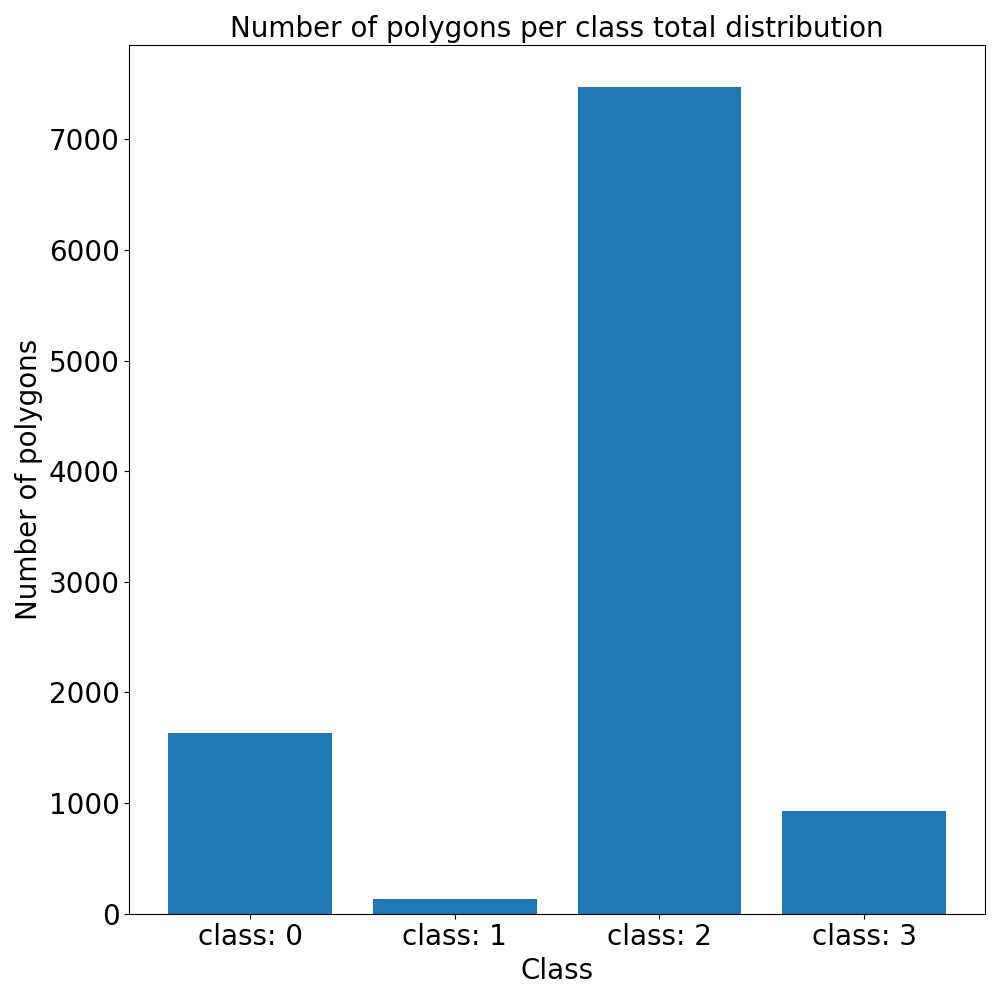
\includegraphics[width=0.35\textwidth]{imgs/Coigan/train_n_polygons_per_class_total_histogram.png}
        }  &
        \subfloat[Distribuzione dei difetti nel test set.]{
            \label{fig:test_sd_polygons_distribution}
            \centering
            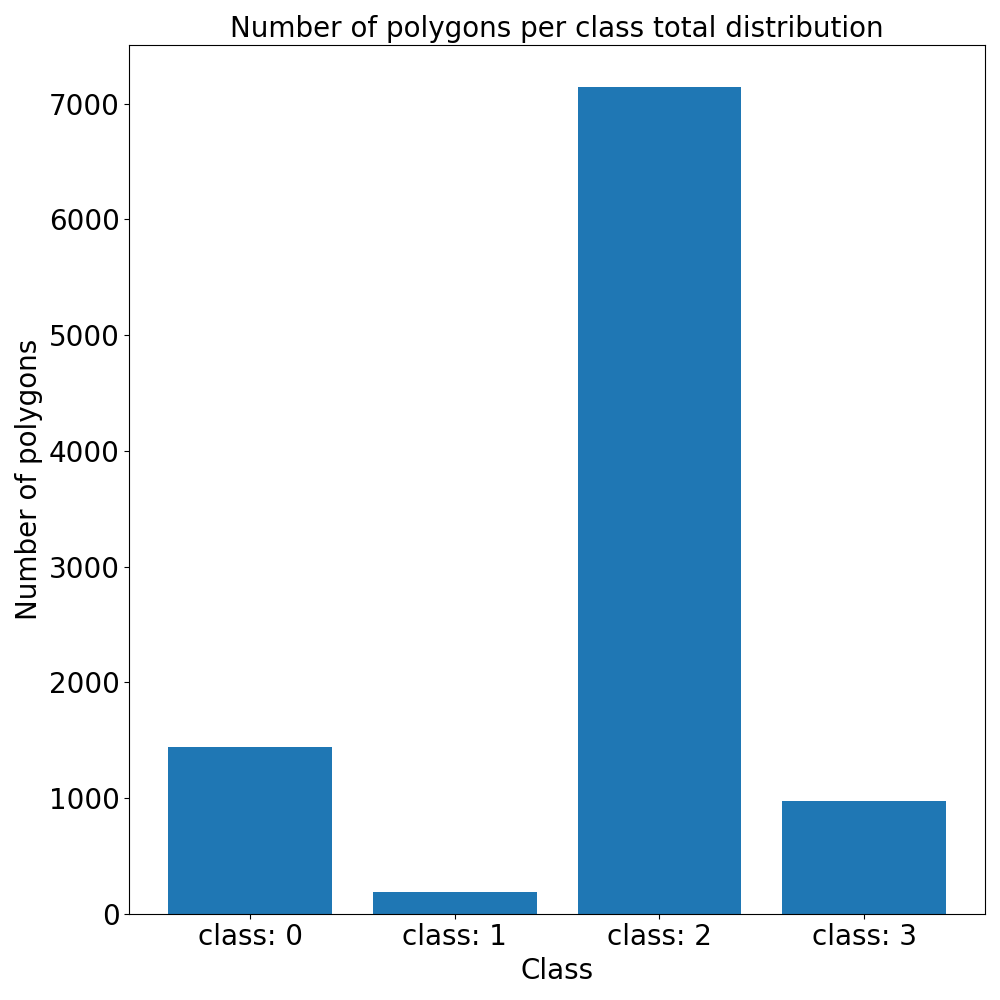
\includegraphics[width=0.35\textwidth]{imgs/Coigan/test_n_polygons_per_class_total_histogram.png}
        }  \\
    \end{tabular}
\end{figure}

% tabella che riassume i valori sopra citati
\begin{table}[H]
    \centering
    \begin{tabular}{|c|c|c|c|c|}
    \hline
            & \textbf{Classe 1} & \textbf{Classe 2} & \textbf{Classe 3} & \textbf{Classe 4} \\
    \hline
    \textbf{Numero di poligoni train set} & 1637 & 130 & 7475 & 931 \\
    \hline
    \textbf{Numero di poligoni test set} & 1445 & 191 & 7147 & 971 \\
    \hline
    \end{tabular}
    \caption{Distribuzione delle immagini per classe.}
    \label{tab:sd_polygons_distribution}
\end{table}


\subsection{Creazione del dataset degli oggetti}
Una volta generato il training set e il test set, per l'addestramento del modello è necessario creare un dataset separato per ogni
classe di difetti i quali contengono esclusivamente i crop dei difetti di quella classe, con le annotazioni relative al crop del difetto.
Si ottengono dunque 4 dataset con immagini quadrate di dimensioni arbitrarie per ognuno dei quali è presente una singola annotazione.

\begin{figure}[H]
    \centering
    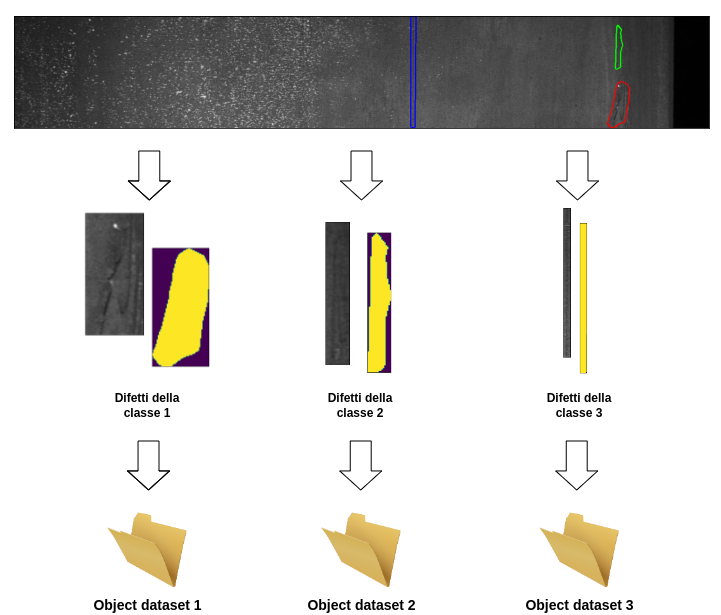
\includegraphics[width=0.8\textwidth]{imgs/Coigan/Object_dataset_generation.drawio.png}
    \caption{Figura che illustra il processo di creazione dei dataset degli oggetti. In questo caso viene mostrato come
    vengono estratti i difetti da una singola immagine contenente 3 difetti, i quali vengono smistati nei rispettivi dataset.}
    \label{fig:object_dataset_generation}
\end{figure}

Per questa tipologia di dataset è stata mantenuto come standard il formato \textit{line json}, ma in quanto in questo caso ad ogni elemento (o immagine) 
corrisponde una sola annotazione è stata modificata la struttura del json, associando ad ogni elemento una lista di punti di un singolo poligono,
ed è stato aggiunto un campo che che indica la dimensione del crop del difetto, tale accortezza permette il caricamento della maschera
senza la necessità di caricare l'immagine per caricare le dimensioni della maschera. Di seguito è mostrato un'esempio di come sono strutturati 
i dati nel formato \textit{line json} per i dataset degli oggetti:

\begin{figure}[H]
    \begin{minted}[
        frame=lines,
        framesep=2mm,
        baselinestretch=1.2,
        bgcolor=light-gray,
        fontsize=\footnotesize,
        linenos
        ]{json}
        {"img": "0.jpg", "points": [[[5, 0], [5, 4], ...]], "shape": [246, 22]}
        {"img": "1.jpg", "points": [[[4, 0], [4, 4], ...]], "shape": [249, 25]}
        ...
    \end{minted}
    \caption{Esempio di file contenente le annotazioni degli object dataset nel formato \textit{line json}.}
\end{figure}

\subsection{Creazione del dataset di immagini base}
\begin{comment}
    Concludi questa parte inderendo il tiling delle immagini con l'algoritmo utilizzato,
    non serve illustrare il codice ma almeno illustrare graficamente la procedura.
\end{comment}
Il dataset di immagini base è utilizzato come base appunto per il processo di inpainting, ed è stato scelto di utilizzare per questo scopo
esclusivamente immagini senza difetti, per semplificare la procedura di addestramento e ridurre il numero di considerazioni da fare.
Infatti utilizzando tutte le immagini del training set come base ci sarebbe stata la possibilità durante il training
di scegliere un'area per la creazione di un difetto che fosse già occupata da un'altro difetto reale con conseguenti disturbi nell'apprendimento.

Un passaggio importante che viene fatto in questa fase, è la procedura di tiling delle immagini, ovvero sono state estratte
7 patch di dimensione 256x256 da ogni immagine, questa scelta è stata guidata principalmente da problematiche legate alla memoria disponibile
per la procedura di training che non avrebbe consentito altrimenti di utilizzare una \textit{batch size} di dimensioni adeguate.
Di seguito in Figura \ref{fig:tiling} vi è un esempio che illustra graficamente come è stata applicata la procedura.\\
Il tilling in questo caso è stato effettuato con un leggero overlap tra le patch, per ottenere delle patch quadrate e
non sprecare nessuna parte dell'immagine.\\

\begin{figure}[H]
    \centering
    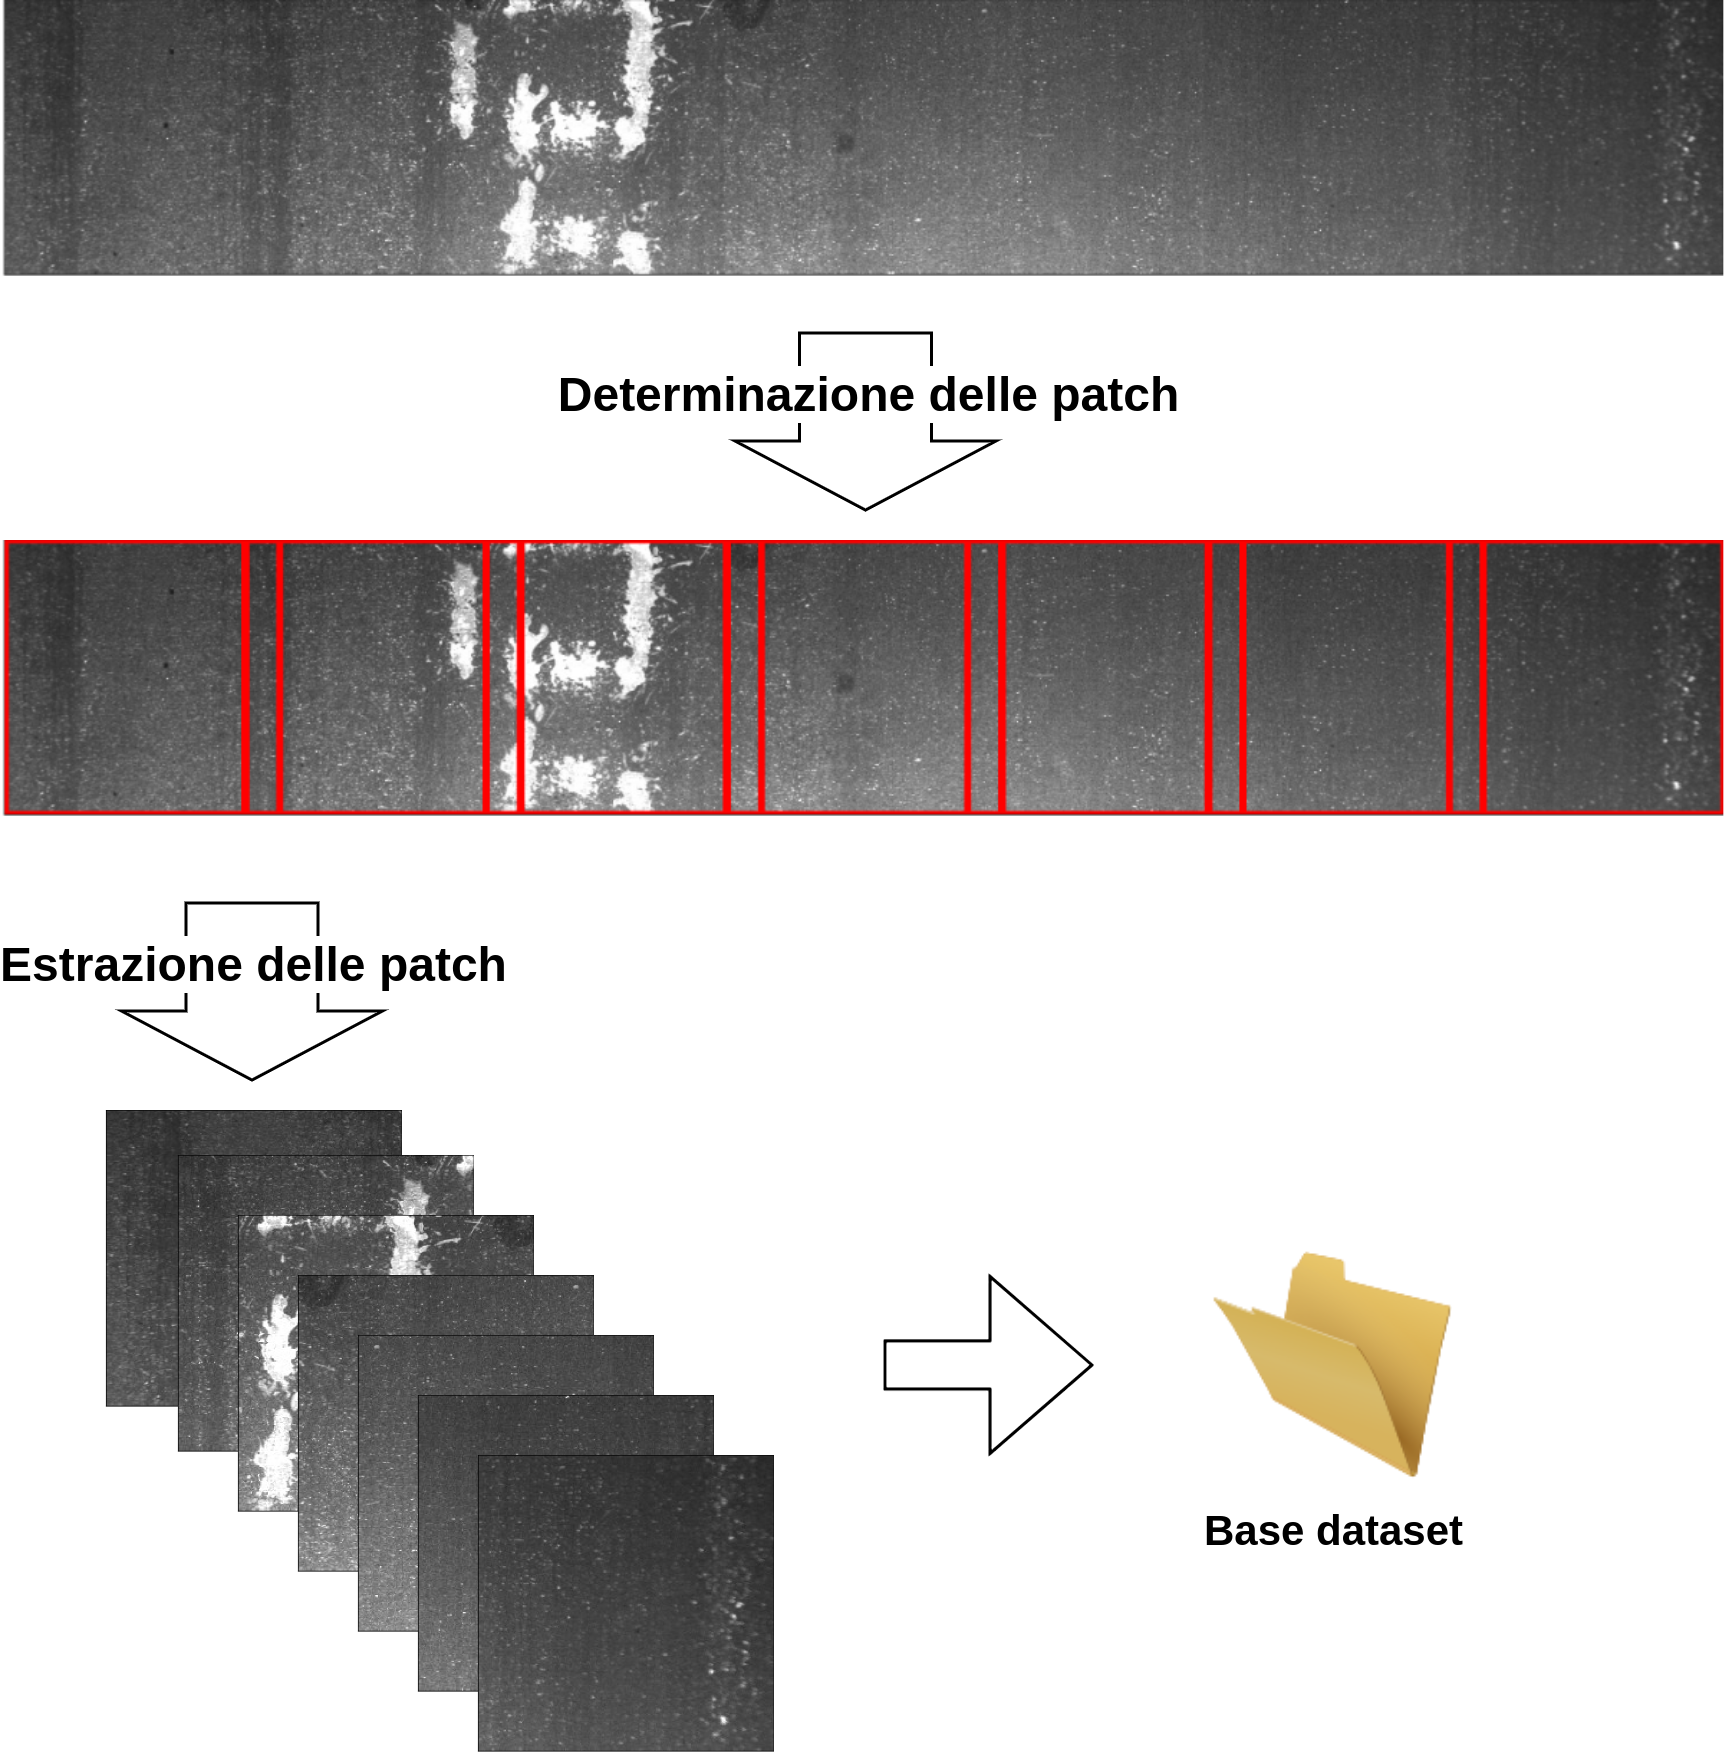
\includegraphics[width=0.85\textwidth]{imgs/Coigan/tilling_op.png}
    \caption{Figura che illustra concettualmente il processo di tiling delle immagini.}
    \label{fig:tiling}
\end{figure}

\subsection{Creazione del dataset utilizzato come riferimento}
Il dataset di riferimento segue la stessa procedura effettuata per il dataset di immagini base, con la differenza che in questo caso
non sono state selezionate immagini specifiche dal training set, ma sono state semplicemente estratte 7 patch di dimensione 256x256 da ogni immagine.
Lo scopo di questo dataset è fornire una distribuzione di riferimento per un discriminatore che confronta le immagini generate con quelle reali,
nella loro interezza, principalmente per cercare di attenuare gli \textit{artifacts} generati dal modello sui bordi dei difetti generati.



\section{Il dataloader}
Il dataloader in questo progetto ha richiesto più lavoro rispetto ad un modello classico di segmentazione o di generazione di immagini,
in quanto doveva gestire 10 sorgenti di dati differenti, le quali poi venivano successivamente combinate, principalmente in tre tensori
utilizzati come input per i vari modelli della pipeline.\\
Data la complessità del dataloader è stato scelto un'approccio modulare, dove ogni componente del dataloader è rappresentata da una classe
che a sua volta incapsula o estende altre classi, in modo da rendere più semplice la gestione delle varie operazioni di caricamento dei dati,
in Figura \ref{fig:dataloader} è mostrato un diagramma UML semplificato del dataloader e delle classi principali che lo compongono, per dare un'idea
della struttura dell'oggetto.\\

In seguito sono discussi le varie componenti del dataloader, con un approccio bottom-up, partendo dalle classi più periferiche e arrivando a descrivere
l'oggetto \textbf{CoiganSeverstalSteelDefectsDataset}, che è l'oggetto che viene incapsulato dall'oggetto \textbf{torch.utils.data.DataLoader}, utilizzato
per effettuare l'addestramento del modello.

\begin{figure}
    \centering
    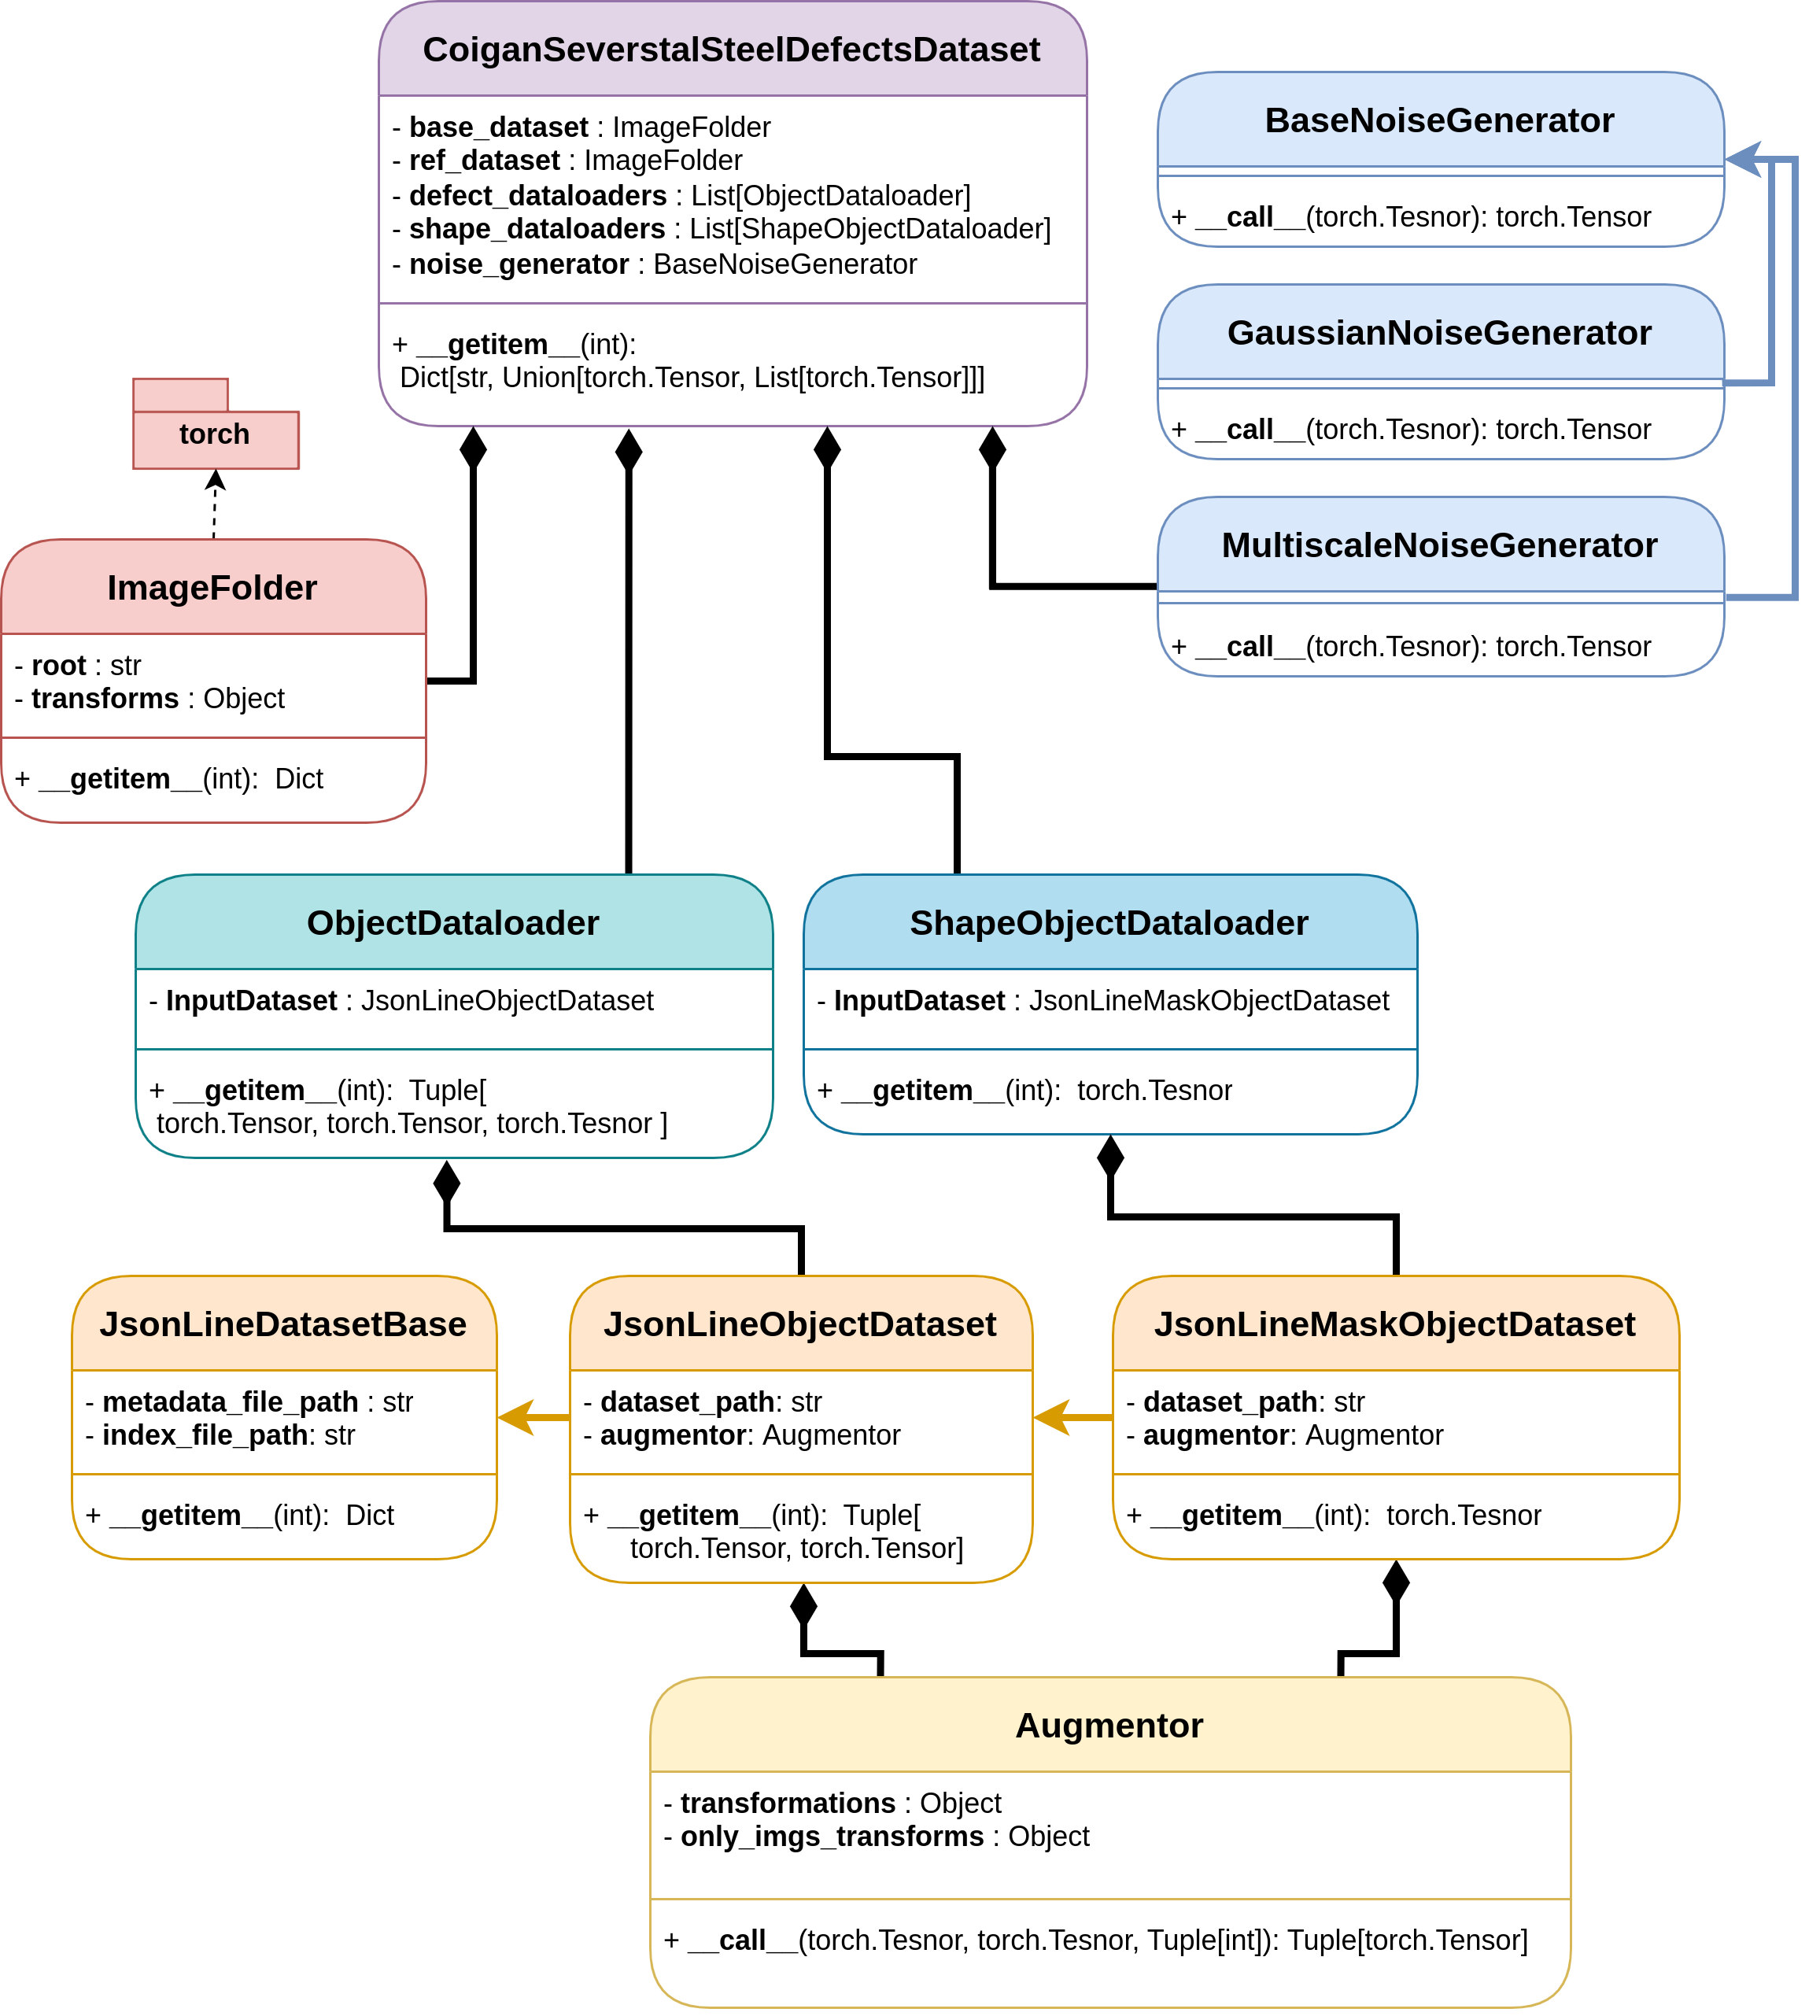
\includegraphics[width=1.0\textwidth]{imgs/Coigan/Dataloader uml.png}
    \caption{In Figura è mostrato il diagramma UML semplificato del dataloader e delle classi principali che lo compongono.
        Questo infatti suddivide diverse operazioni di caricamento dei dati in classi separate, le quali fanno convergere i risultati
        all'oggetto \textbf{CoiganSeverstalSteelDefectsDataset} che restituisce un output compatibile con l'oggetto \textbf{torch.utils.data.DataLoader}.}
    \label{fig:dataloader}
\end{figure}



\subsection{L'oggetto Augmentor}
L'oggetto Augmentor è stato realizzato per permettere una gestione agevole delle operazioni di \textit{data augmentation} da applicare a
immagini e maschere, in quanto queste necessitano di essere trattate in maniera differente per quanto riguarda alcune specifiche augmentation,
mentre per altre necessitano di mantenere una coerenza tra maschera e immagine.\\

Vediamo due casi che chiariscono la necessità di questa divisione, il primo caso potrebbe essere una rotazione di un angolo arbitrario,
applicando separatamente la rotazione ad un'immagine e alla sua maschera, quest'ultima non avrebbe più alcuna coerenza con l'immagine,
per tale ragione questo tipo di operazione viene effettuata in maniera sincrona, ovvero applicando la stessa rotazione sia all'immagine che alla maschera.\\
Per quanto riguarda il secondo caso, possiamo considerare un'operazione di aggiustamento del contrasto, sull'immagine questa operazione può essere
applicata senza problemi ma passando la maschera a tale trasformazione si otterrebbe un errore, in quanto la maschera è una matrice binaria, con un solo canale,
tali considerazioni valgono per ogni altra trasformazione nello spazio dei colori, e in quello della morfologia delle immagini e delle maschere.

Per risolvere tali problematiche sono stati creati degli oggetti che estendono \textbf{torch.nn.Module}, e che seguendo la medesima struttura degli oggetti
\textit{transformation} presenti nel pacchetto \textbf{torchvision.transforms}, applicano le trasformazioni alle immagini e alle maschere in batch, tali metodi
sono presenti nel file \path{COIGAN/training/data/augmentation/custom_transformations.py}.\\
Come è possibile vedere dal diagramma UML infatti, l'oggetto Augmentor accetta due liste di oggetti \textbf{torch.nn.Module}, una per le trasformazioni
che verranno applicate esclusivamente alle immagini, e una per le trasformazioni che verranno applicate alle maschere e alle immagini.\\

Una peculiarità di questo oggetto è che consente oltre alle trasformazioni di \textit{data augmentation} anche di applicare delle trasformazioni
fisse alla dimensione dei tensori dopo l'augmentation, così da poter adattare le immagini all'input di un modello con dimensione fissa, o semplicemente
permettendo di avere tensori della stessa dimensione che possono essere impilati per formare dei batch, in base al caso d'uso.



\subsection{Gli oggetti JsonLineObjectDataset e JsonLineMaskObjectDataset}
Il primo layer tra i dati e l'interfaccia finale del dataloader, è rappresentato da due oggetti: \textbf{JsonLineObjectDataset} e \textbf{JsonLineMaskObjectDataset}.
Questi due oggetti che fungono da dataloader intermedi, vengono utilizzati per il caricamento dei dataset dei difetti, 
i quali sono in formato \textit{line json}, come precedentemente descritto.

Entrambi i dataloader discendono dalla classe \textbf{JsonLineDatasetBase}, la quale presenta le primitive per il caricamento dei dataset in formato \textit{line json},
binario e non, senza alcun preconcetto su quale debba essere la struttura degli esempi contenuti al suo interno, dunque potenzialmente utilizzabile per qualunque tipo di dataset
basato su questa struttura.

La prima estensione di questa classe è data da \textbf{JsonLineObjectDataset}, la quale estende la classe base aggiungendo la funzionalità di caricamento
dei dati contenuti negli esempi, ovvero non solo è in grado di caricare i metadati ma anche anche di caricare l'immagine dell'oggetto e la relativa maschera binaria come \textbf{torch.Tensor},
in quanto il \textbf{JsonLineObjectDataset} si aspetta una determinata struttura all'interno dei sample ottenuti dai metodi della classe madre \textbf{JsonLineDatasetBase}.
In fine l'oggetto \textbf{JsonLineMaskObjectDataset} estende \textbf{JsonLineObjectDataset} effettuando un override del metodo \textbf{\_\_getitem\_\_$()$} per restituire esclusivamente la maschera
senza effettuare il caricamento dell'immagine, in quanto questo oggetto è utilizzato nei i casi in cui l'immagine RGB non è necessaria.

Entrambi questi oggetti accettano come argomento del costruttore un oggetto \textbf{Augmentor} preconfigurato, il quale viene utilizzato per applicare le trasformazioni
agli esempi caricati, direttamente durante l'operazione di caricamento, così da avere in uscita da tali oggetti gli esempi con l'\textit{augmentation} già applicata.



\subsection{L'oggetto ObjectDataloader e ShapeObjectDataloader}
Un'ulteriore layer di astrazione tra l'uscita del dataloader e i dati sono gli oggetti \textbf{ObjectDataloader} e \textbf{ShapeObjectDataloader}, questi due infatti
vengono caricati nel oggetto \textbf{CoiganSeverstalSteelDefectsDataset} e vengono utilizzati per supportare la creazione degli effettivi tensori di uscita.
Lo scopo di questi oggetti è quello di caricare i difetti provenienti dai dataset degli oggetti precedentemente menzionati e di posizionarli in dei tensori delle dimensioni adatte alla pipeline di training
in maniera casuale, evitando di posizionarli in sovrapposizione ad altri difetti nello stesso tensore.\\
I due oggetti del dataloader si differenziano principalmente per il fatto che \textbf{ObjectDataloader} carica le immagini dei difetti e le loro maschere restituendo un tensore per entrambi, mentre lo 
\textbf{ShapeObjectDataloader} carica solamente le maschere restituendo un unico tensore.
Di seguito in figura \ref{fig:object_dataloader_sample} un esempio di come i difetti vengono caricati dal \textbf{JsonLineObjectDataset} e poi vengono trasformati dal \textbf{ObjectDataloader}.

\begin{figure}[H]
    \centering
    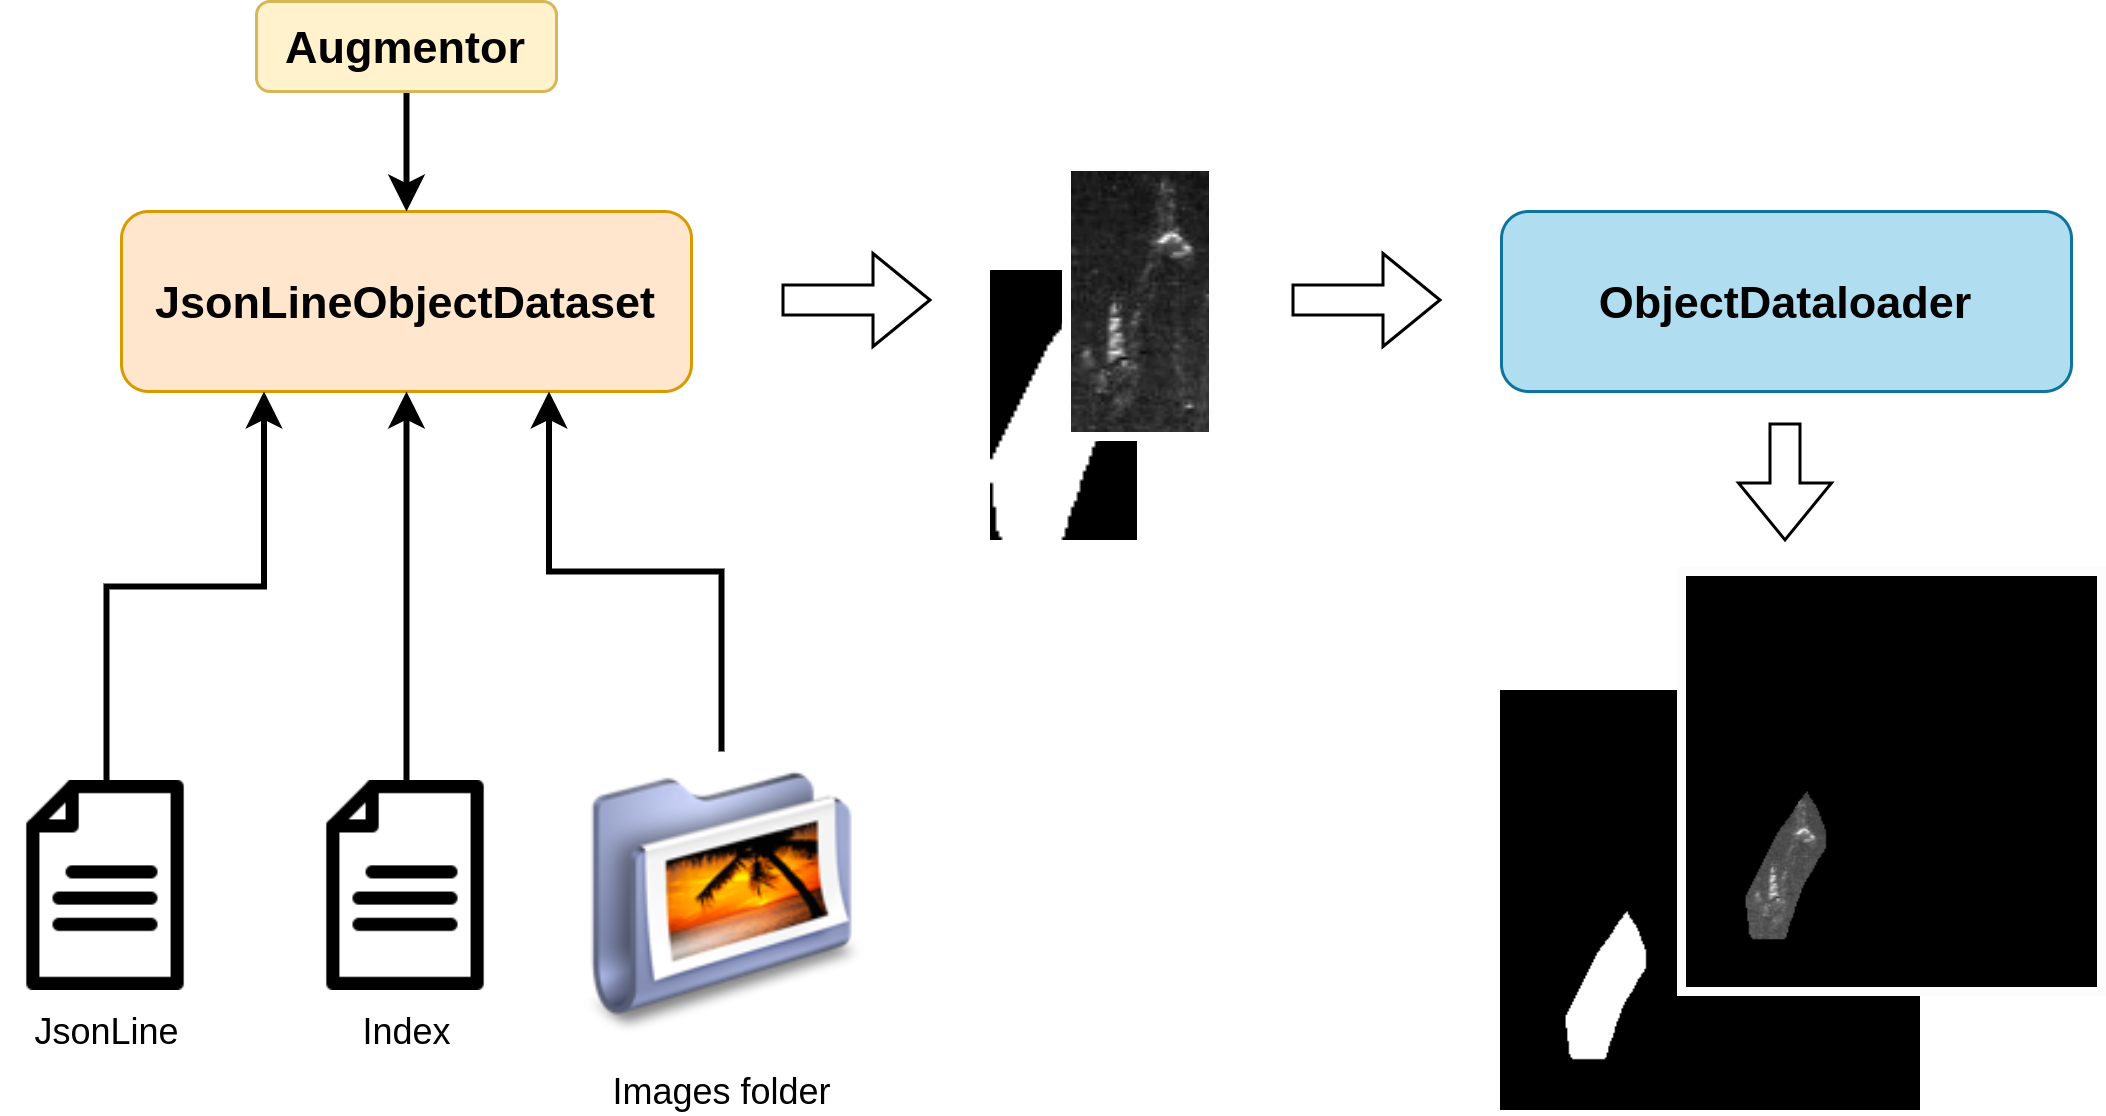
\includegraphics[width=1.0\textwidth]{imgs/Coigan/Dataloader_pipeline_example.drawio.png}
    \caption{Figura che illustra concettualmente il processo di caricamento degli oggetti da parte del \textbf{ObjectDataloader}.}
    \label{fig:object_dataloader_sample}
\end{figure}


\subsection{L'oggetto ImageFolder}
La classe ImageFolder è una classe fornita da PyTorch per gestire dataset di immagini in modo semplice ed efficiente. 
È progettata per lavorare con dataset che seguono una struttura a directory, ed è principalmente utilizzata per dataset di classificazione.
La struttura delle directory richiesta da ImageFolder è la seguente:

\begin{itemize}
    \item root/class\_1/sample\_1.png
    \item root/class\_1/sample\_2.png
    \item ...
    \item root/class\_2/sample\_1.png
    \item root/class\_2/sample\_2.png
    \item ...
\end{itemize}

Dove root è la directory principale del dataset e class\_1, class\_2, ecc., sono le sottodirectory che rappresentano le diverse classi di immagini nel dataset.
Quando si crea un'istanza della classe ImageFolder, è necessario specificare il percorso alla directory principale del dataset come argomento
e il caricamento delle immagini con l'assegnazione delle classi viene effettuato automaticamente.
Nel caso di COIGAN è stata utilizzata una sola classe, in quanto l'obbiettivo era semplicemente caricare delle immagini in formato \textbf{torch.Tensor}.



\subsection{Il Noise Generator}
Il Noise generator è un oggetto che viene utilizzato all'interno di \textbf{CoiganSeverstalSteelDefectsDataset} per introdurre del
rumore nelle maschere di input del generatore, dove ci si aspetta che il generatore vada a generare dei difetti sull'immagine di input.\\
L'architettura scelta (vedi \ref{sec:lama}) prevede che il generatore riceva in input un'immagine e delle maschere ma
non ha nessun ingresso preferenziale per il rumore, per tale ragione questo viene introdotto 
direttamente nelle maschere di input, per garantire una buona variabilità dell'output.\\
Le classi figlie dell'interfaccia \textbf{BaseNoiseGenerator}, ovvero: \textbf{GassianNoiseGenerator} e \textbf{MultiscaleNoiseGenerator},
implementano due metodi di immissione del rumore differenti ma in sintesi, entrambi prendono in ingresso un tensore contenente una maschera
binaria e restituiscono un tensore della stessa dimensione con del rumore applicato in corrispondenza dei pixel con valore 1 nella maschera.

Il \textbf{GassianNoiseGenerator} è un generatore molto semplice che applica del rumore gaussiano con media e deviazione standard configurabili
in corrispondenza dei pixel con valore 1 nella maschera, come mostrato in Figura \ref{fig:gaussian_noise}.

\begin{figure}[H]
    \centering
    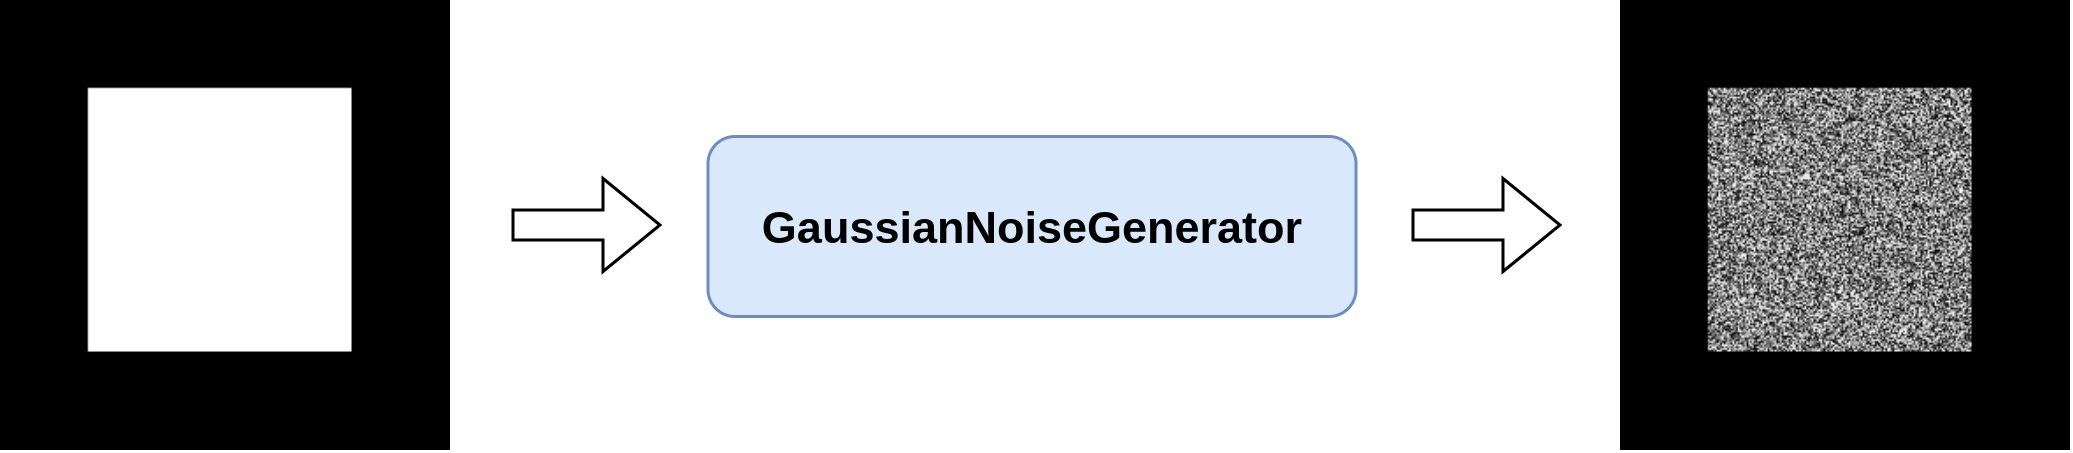
\includegraphics[width=0.8\textwidth]{imgs/Coigan/gaussian noise generator.drawio.png}
    \caption{Figura che illustra un esempio di applicazione del \textbf{GassianNoiseGenerator}.}
    \label{fig:gaussian_noise}
\end{figure}

Il \textbf{MultiscaleNoiseGenerator} invece è un generatore più articolato il quale può ospitare al suo interno un'ulteriore 
generatore di rumore, ed è in grado di applicare il rumore proveniente dal generatore interno a diverse scale per dare una variabilità più realistica al rumore applicato.
Per ottenere tale effetto date $n$ scale, ad esempio [1, 8, 16], dato un tensore di ingresso di dimensioni $h$ $w$, il generatore crea 3 tensori di rumore con rispettivamente
dimensioni $h$ $w$, $\frac{h}{8}$ $\frac{w}{8}$ e $\frac{h}{16}$ $\frac{w}{16}$, e riporta tramite interpolazione bilineare tutti i tensori alla dimensione $h$ $w$,
per poi sommarli, come è illustrato nella figura \ref{fig:multiscale_noise_generation}.

\begin{figure}[H]
    \centering
    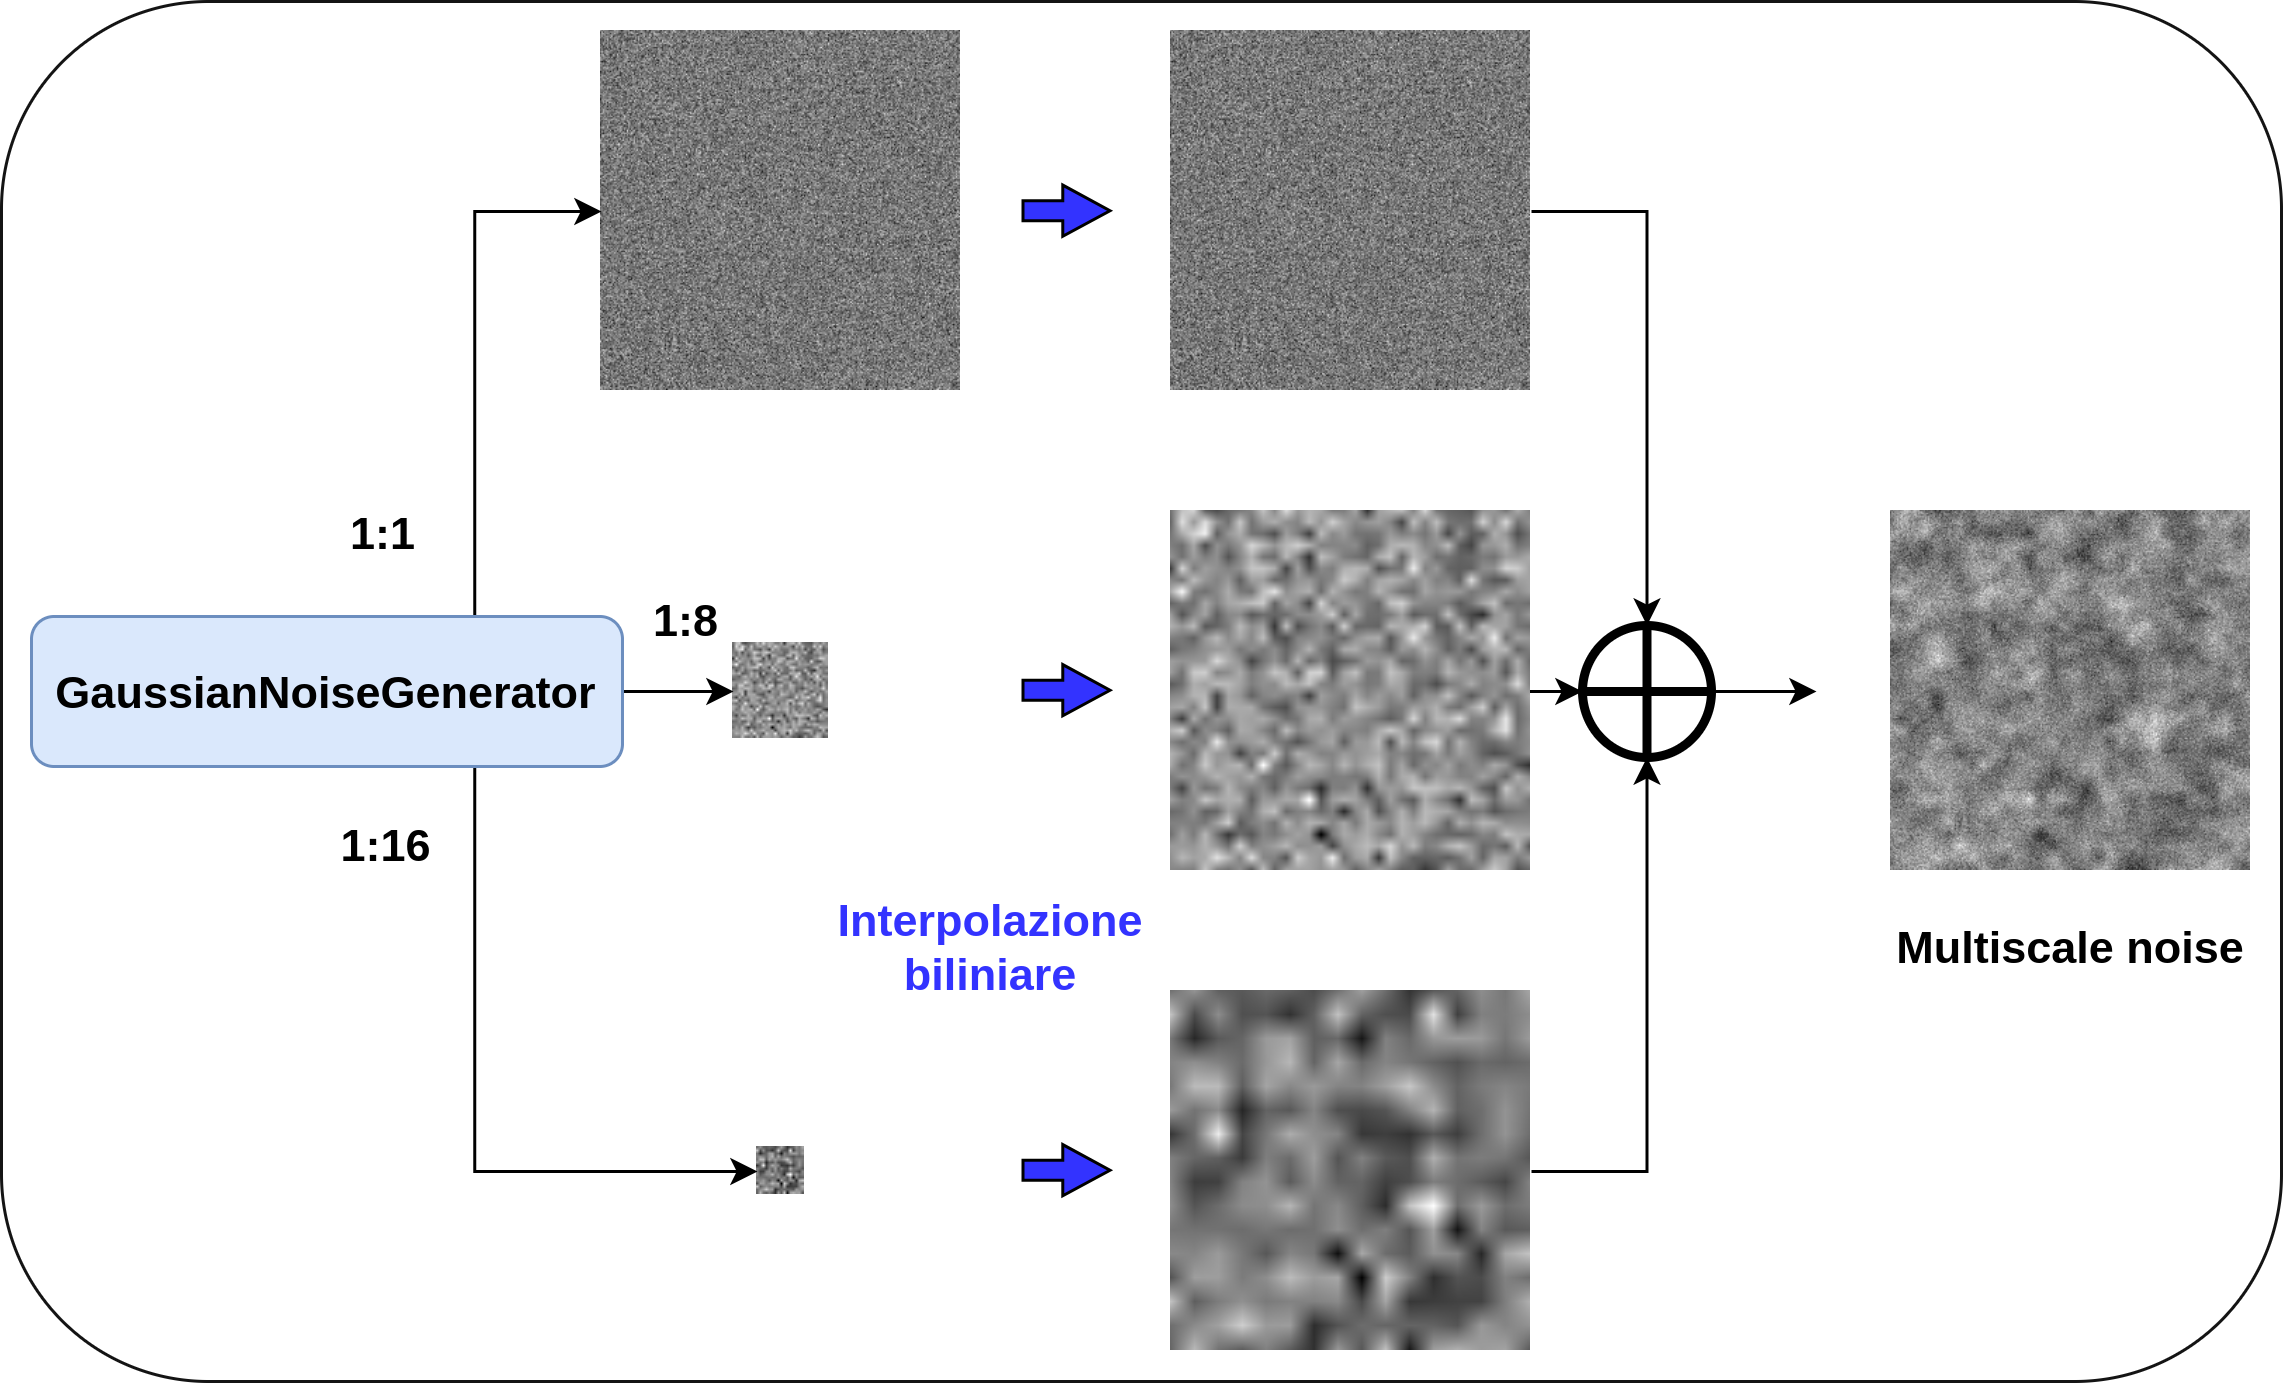
\includegraphics[width=0.9\textwidth]{imgs/Coigan/Multiscale_noise/Multiscale_noise_generation.png}
    \caption{Figura che illustra un esempio di generazione di rumore all'interno del \textbf{MultiscaleNoiseGenerator}.}
    \label{fig:multiscale_noise_generation}
\end{figure}

Per mitigare l'effetto di discontinuità tra le aree dell'output del modello in cui viene richiesta la generazione di un 
difetto e le aree circostanti, le quali tendevano a generare degli artifacts durante i primi addestramenti è stata introdotta un'ulteriore
\textit{feature} al \textbf{MultiscaleNoiseGenerator}, ovvero la possibilità di applicare un smooth gaussiano alla maschera prima di applicare il rumore.
Tale tecnica consente una attenuazione graduale del rumore allontanandosi dal difetto, contribuendo a mitigare gli artifacts in tali aree.
Nella figura \ref{fig:multiscale_noise_application} è possibile vedere un esempio di come viene applicato lo smoothing e il rumore generato nel passaggio precedente
alla maschera in ingresso.

\begin{figure}[H]
    \centering
    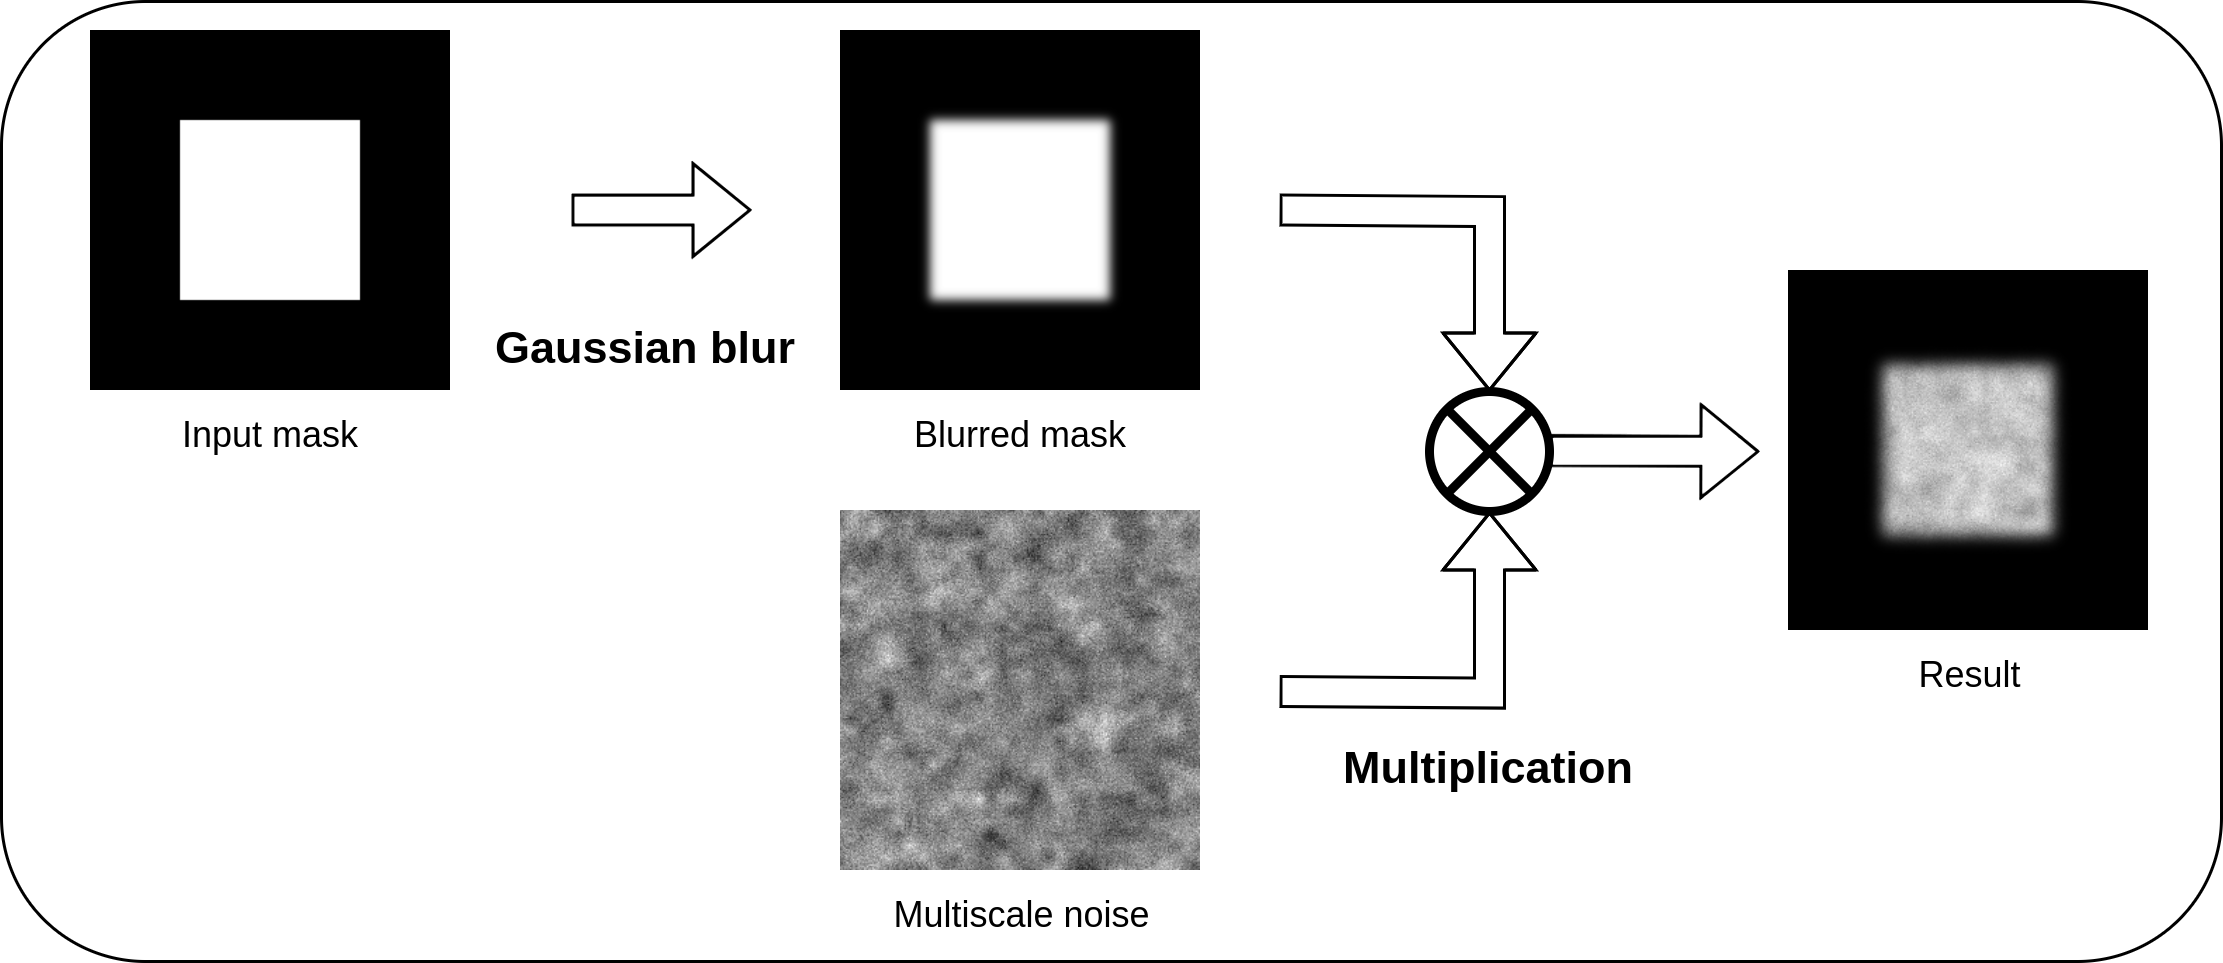
\includegraphics[width=0.9\textwidth]{imgs/Coigan/Multiscale_noise/Multiscale_noise_application.png}
    \caption{Figura che illustra un esempio di applicazione del rumore generato dal \textbf{MultiscaleNoiseGenerator}.}
    \label{fig:multiscale_noise_application}
\end{figure}

\subsection{L'oggetto CoiganSeverstalSteelDefectsDataset}
\begin{comment}
In questa sezione devo discutere dell'utilizzo dell 'oggetto CoiganSeverstalSteelDefectsDataset,
che in pratica prende tutti i dataloader di ogni dataset e riaggrega i dati in uscita da questi in una serie di oggetti utili
alla pipeline di addestramento. 

lista delle operazioni svolte dall'oggetto:
- estrazione di un'immagine base dal dataset delle immagini base
- estrazione di un'immagine di riferimento dal dataset di riferimento
- estrazione di un'immagine contenente difetti dall'ObjectDataloader per ogni classe
- estrazione di una maschera contenente difetti dal ShapeObjectDataloader per ogni classe
- se richiesto effettua il masking della base image
- applica il rumore alle maschere di input del generatore
- effettua la concatenazione dei tensori per creare i tensori di input per il generatore e i discriminatori
- ritorna i tensori
\end{comment}

L'oggetto \textbf{CoiganSeverstalSteelDefectsDataset} dunque è un contenitore che si occupa di caricare tutti i dati pre-elaborati dai
vari dataloader concatenandoli dove necessario, applicando in oltre alcune modifiche finali ai tensori da passare alla pipeline di addestramento.

Abbiamo visto dunque dallo schema UML e per quanto detto precedentemente che questo oggetto raggruppa 6 dataloader differenti, ovvero 2 \textbf{ImageFolder},
uno per il dataset delle immagini base e uno per le immagini da riferimento per uno dei discriminatori, mentre ha ben 4 dataloader differenti per i dataset degli oggetti,
uno per ogni classe, i quali come visto caricano le immagini e le maschere degli oggetti, tali difetti vengono poi utilizzati per addestrare il discriminatore dei difetti,
mentre le maschere sono utilizzate anche come input per il generatore. Tale configurazione è mostrata nella figura \ref{fig:coigan_severstal_steel_defects_dataset_sample}.

\begin{figure}[H]
    \centering
    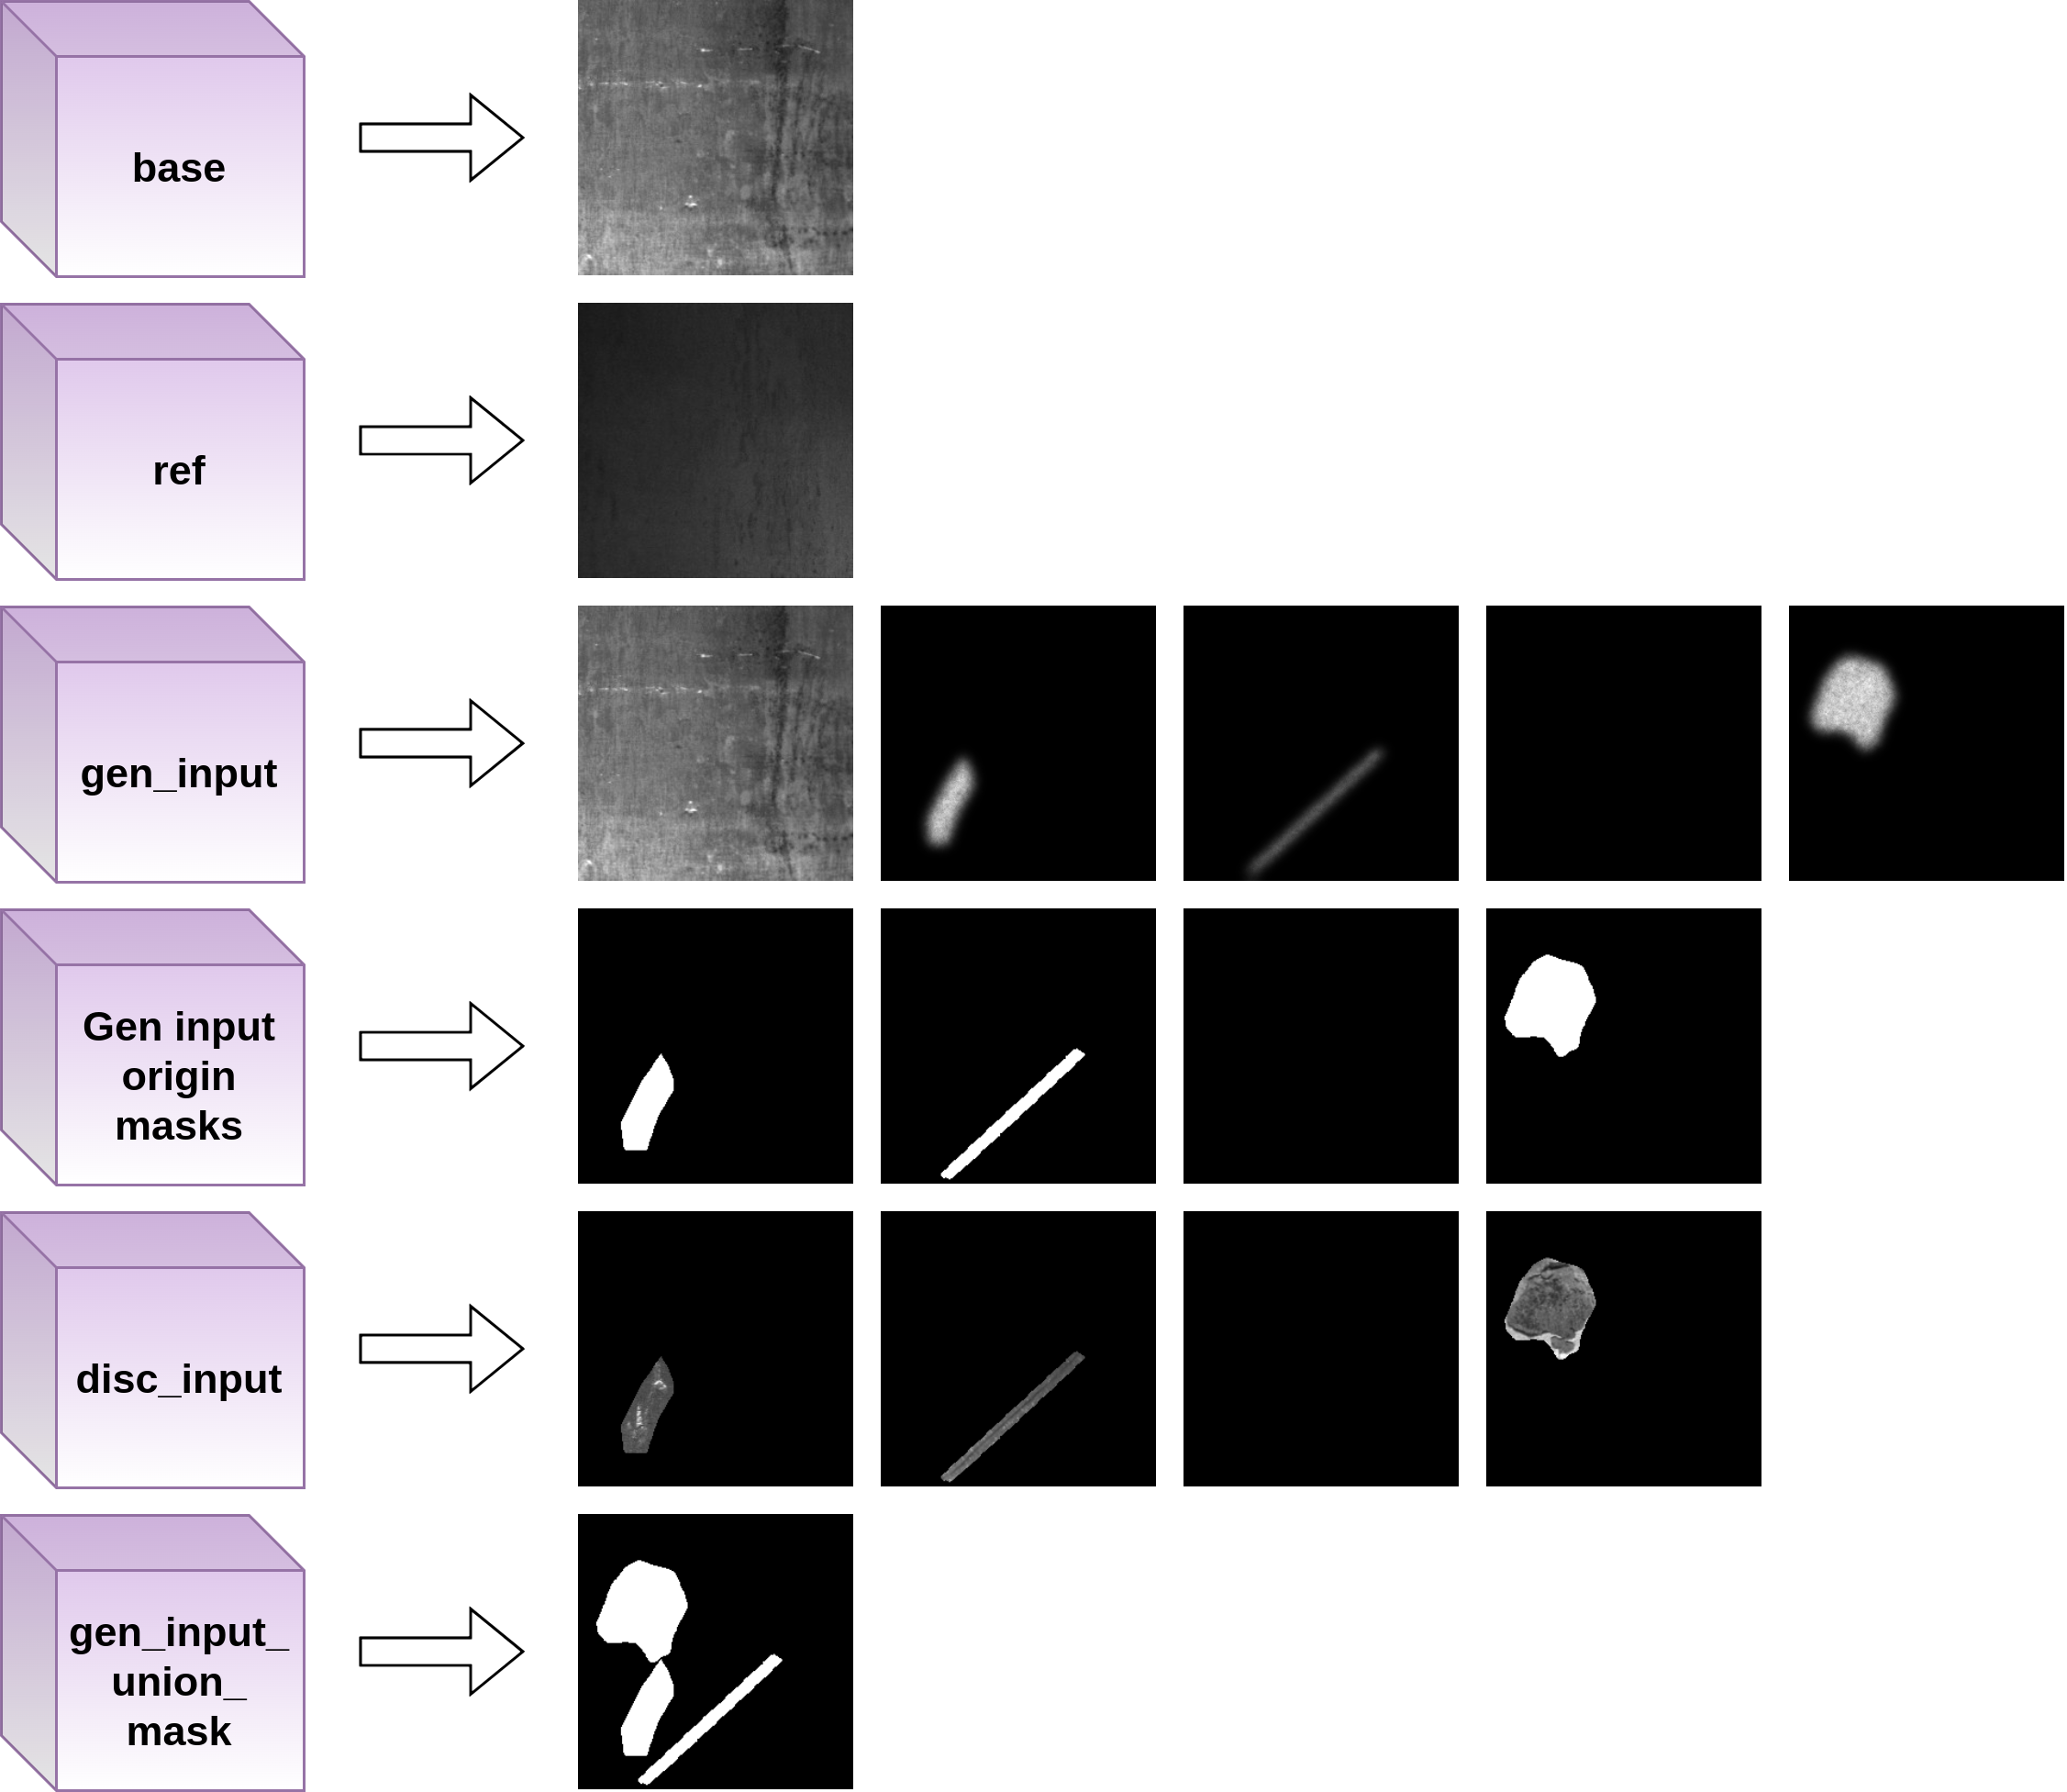
\includegraphics[width=0.9\textwidth]{imgs/Coigan/Output_coigan_dataloader.png}
    \caption{Nella figura è mostrato il contenuto di un sample che si può ottenere dall'oggetto \textbf{CoiganSeverstalSteelDefectsDataset},
    a sinistra i cubi rappresentano i tensori, con i nomi effettivi che sono presenti nel dict, mentre a destra vi sono i canali dei tensori,
    le immagini raggruppano 3 canali mentre le maschere occupano un solo canale. Si noti che l'ordine da sinistra verso destra è coerente
    con l'ordine dei canali nei tensori.}
    \label{fig:coigan_severstal_steel_defects_dataset_sample}
\end{figure}

Con un'impostazione però è possibile richiedere maschere di input diverse dai difetti passati al discriminatore, arrivando a 10 dataloader differenti, in quanto
si aggiungono ulteriori 4 dataloader per la generazione delle maschere di input, le quali verranno generate da dei dataloader \textbf{ShapeObjectDataloader} che caricano
esclusivamente le maschere degli oggetti e non le immagini, anche se effettuano la lettura degli stessi dataset.

L'oggetto restituito dal \textbf{CoiganSeverstalSteelDefectsDataset} come sample è un \textit{dict} che associa delle stringhe a dei tensori, tali tensori sono illustrati in
figura \ref{fig:coigan_severstal_steel_defects_dataset_sample} dove i nomi sui cubi che rappresentano i tensori sono gli effettivi nomi utilizzati nel dict.
Verra poi illustrato come questi tensori vengono utilizzati nella pipeline di addestramento nella prossima sezione.

In sintesi vediamo le operazioni svolte da questo oggetto:

\begin{itemize}
    \item Estrae un'immagine base dal dataset delle immagini base.
    \item Estrae un'immagine di riferimento dal dataset di riferimento.
    \item Estrae delle immagini e delle maschere dei difetti dall'\textbf{ObjectDataloader} per ogni classe.
    \item Estrae delle maschere dei difetti dallo ShapeObjectDataloader per ogni classe, se specificato nelle configurazioni altrimenti riutilizza le maschere caricate in precedenza.
    \item Se richiesto effettua il masking della base image, con le maschere dei difetti che verranno passate in input al generatore.
    \item Applica il rumore alle maschere di input del generatore.
    \item Effettua la \textit{stack} dei tensori per creare i tensori di input per il generatore e i discriminatori.
    \item Ritorna i tensori come dict.
\end{itemize}

il dict restituito da questo oggetto viene poi processato dal \textbf{torch.utils.data.DataLoader}, il quale oltre a gestire il caricamento dei dati, 
si occupa anche di creare i batch, e di gestire il caricamento tramite istanze multiple di questo oggetto utilizzando il \textit{multiprocessing} di Python.

\section{La pipeline di addestramento}
\begin{comment}
Questa sezione verra divisa in:

    - il generatore (in generale) e la path-length regularization
    - il discriminatore dei difetti e la sua loss e la R1 regularization
    - il discriminatore delle immagini e la sua loss
    - la perceptual loss e la rete preaddestrata utilizzata
    - la l1 loss

    Forse non dovrei cercare di dividere le componenti ma discutere un blocco con tutte le sue 

\end{comment}

In questa sezione verranno illustrate nel dettaglio le componenti della pipeline di addestramento, mostrando effettivamente come vengono utilizzati 
i dati caricati dal dataloader precedentemente mostrati, verrà mostrato come vengono calcolate e utilizzate le loss, 
e le regolarizzazioni per l'addestramento dei modelli.

\subsection{Il generatore}
Il generatore è la componente principale della pipeline, e come già detto utilizza la medesima architettura di LaMa, l'unica modifica che
è stata apportata alla struttura del modello è la dimensione del tensore di ingresso il quale può variare in base al numero di classi di oggetti che
si vogliono generare.\\
La loss di questo modello è composta da 4 elementi come mostrato nella figura \ref{fig:pipeline_di_addestramento} più la regolarizzazione, ovvero: le non saturating loss 
calcolate con l'output dei discriminatori, la perceptual loss, la L1 e in fine la \textit{path-length regularization}.\\
In questa parte andiamo ad analizzare in dettaglio come sono state implementate la \textit{non saturating loss}, la \textit{path-length regularization} e la L1 loss,
mentre la perceptual loss varrà discussa in seguito.

\subsubsection{La non saturating loss}
Nella loss totale del generatore sono presenti due componenti relative al discriminatore dei difetti e al discriminatore delle immagini, per i quali si utilizza la 
\textit{non saturating loss} come nella paper originale di Goodfellow \cite{goodfellow2014generative}, la quale nel codice è definita come segue:

%python code
\begin{minted}[
    frame=lines,
    framesep=2mm,
    baselinestretch=1.2,
    bgcolor=light-gray,
    fontsize=\footnotesize,
    linenos
    ]{python}
    def g_nonsaturating_loss(discriminator_output):
        return loss = F.softplus(-discriminator_output).mean()
\end{minted}

Tale formulazione della \textit{non saturating loss} è comprensiva della funzione di attivazione sigmoide, 
in quanto i modelli dei discriminatori non ne sono provvisti, infatti abbiamo:

%sigmoide
\begin{equation}
    \sigma(x) = \frac{1}{1 + e^{-x}}
    \label{eq:sigmoid}
\end{equation}

\begin{equation}
    softplus(x) = \log(1 + e^{x})
    \label{eq:softplus}
\end{equation}

%generator non saturating loss classic
\begin{equation}
    L_{G}(D) = \mathbb{E}_{z \sim p_{z}(z)}[ - \log(\sigma(D(G(z))))] = \mathbb{E}_{z \sim p_{z}(z)}[softplus(-D(G(z)))]
    \label{eq:generator_nonsaturating_loss_softplus}
\end{equation}

é possibile notare come la concatenazione della sigmoide \ref{eq:sigmoid} e dalla \textit{non saturating loss} sia equivalente alla 
funzione \textit{softplus} \ref{eq:softplus} applicata all'output del discriminatore, come mostrato in \ref{eq:generator_nonsaturating_loss_softplus}.

\subsubsection{La loss L1 smooth masked}
Per quanto riguarda la L1 loss, come accennato all'inizio di questo capitolo, è stata implementata una versione modificata,
chiamata \textbf{L1 smooth masked}, questa loss viene applicata per calcolare la differenza tra l'immagine generata e l'immagine base
utilizzata per l'inpainting, pesando in maniera differente le aree dove è stato effettuato l'inpainting e le aree 
dove l'immagine deve combaciare con l'immagine base.\\
Rispetto all'implementazione originale presente in LaMa è stata aggiunta una convoluzione della maschera utilizzata per il calcolo dei pesi delle
varie aree, tale tecnica è stata utilizzata per mitigare la formazione di artifacts nelle aree di transizione tra le aree in cui è stato effettuato l'inpainting e non.\\
Vediamo di seguito il metodo che applica la loss L1 smooth masked:

\begin{minted}[
frame=lines,
framesep=2mm,
baselinestretch=1.2,
bgcolor=light-gray,
fontsize=\footnotesize,
linenos
]{python}

    def __call__(self, pred, target, mask):
        """
        Args:
            pred (torch.Tensor): prediction tensor
            target (torch.Tensor): target tensor, reference for the prediction
            mask (torch.Tensor): mask tensor, with values in {0, 1}, 
                where 1 means the pixel correspond to an impainted area.
        """

        # create the smoothed mask
        if self.kernel_size > 0:
            mask = F.conv2d(mask, self.kernel, padding=self.kernel_size // 2)

        # convert the mask in a weight mask
        weight_mask = self.obj_weight * mask + self.bg_weight * (1 - mask)

        # apply the masked L1 loss
        loss = F.l1_loss(pred, target, reduction='none')
        loss = loss * weight_mask

        return loss.sum() / weight_mask.sum()
\end{minted}

Quello mostrato è il metodo \_\_call\_\_ della classe \textbf{SmoothMaskedL1} presente nel file \path{COIGAN/training/losses/masked_losses/smooth_masked_l1.py},
il quale effettua i seguenti passaggi:

\begin{itemize}
    \item \textbf{Riga 13:} Effettua lo smoothing della maschera in ingresso, che indica le aree in cui è stato effettuato l'inpainting, utilizzando una convoluzione 2D.
    \item \textbf{Riga 16:} Effettua la conversione della maschera in un tensore di pesi, dove i pixel con valore 1 nella maschera vengono moltiplicati per il peso
        assegnato alle aree in cui è stato effettuato l'inpainting, mentre la maschera invertita viene moltiplicata per il peso assegnato al resto dell'immagine.
    \item \textbf{Riga 19:} Applica la L1 loss tra l'immagine generata e l'immagine base, senza effettuare la riduzione, in modo da ottenere un tensore di loss
        con la stessa dimensione dell'immagine.
    \item \textbf{Riga 20:} Moltiplica il tensore della loss per il tensore dei pesi, in modo da pesare in maniera differente la loss associata alle diverse aree.
    \item \textbf{Riga 22:} Effettua la riduzione della loss, dividendo la somma del tensore di loss per la somma del tensore di pesi,
        in modo da ottenere una loss normalizzata rispetto ai pesi.
\end{itemize}

Vediamo di seguito la figura \ref{fig:l1_smooth_masked_example} la quale illustra graficamente i passaggi della loss L1 smooth masked, applicati ad un'immagine 
esempio alla quale simuliamo di applicare l'inpainting dove è specificato da una maschera binaria, per simulare il processo è stato applicato del rumore gaussiano
su tale punto, ed è si è utilizzato un peso di 1.0 per il background mentre si è utilizzato un peso di 0.0 per l'area indicata dalla maschera, e si è utilizzato un
kernel di dimensione 5x5 per lo smoothing della maschera.

\begin{figure}[H]
    \centering
    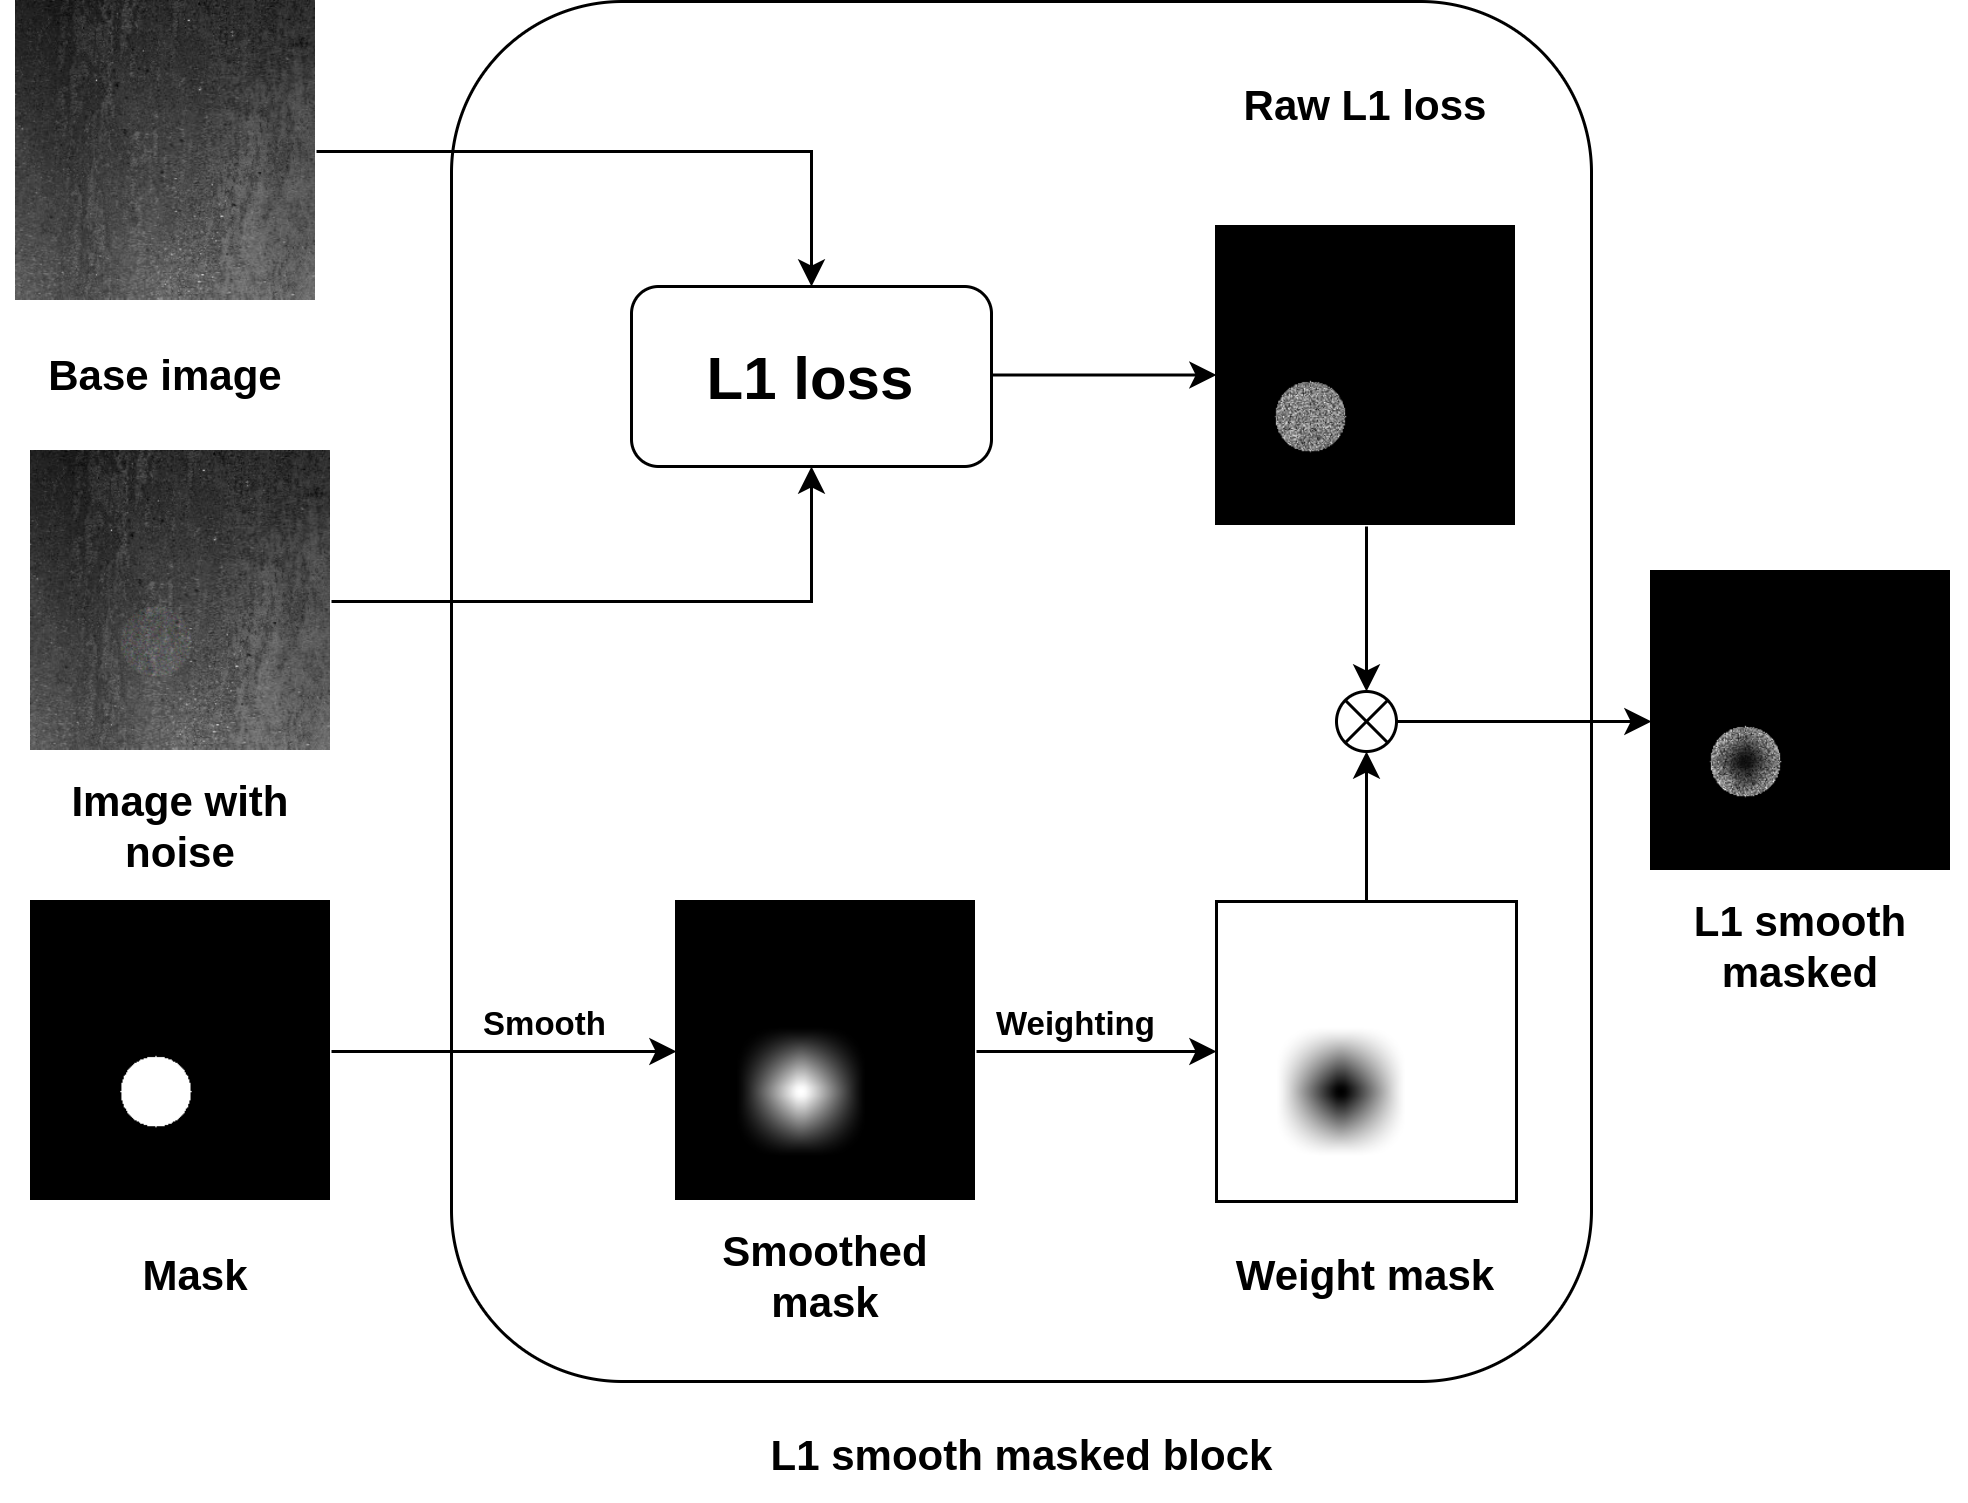
\includegraphics[width=0.9\textwidth]{imgs/Coigan/L1_smooth_masked.png}
    \caption{Figura che illustra graficamente il processo di calcolo della loss L1 smooth masked.}
    \label{fig:l1_smooth_masked_example}
\end{figure}

Il risultato di questa operazione è che anche un'area localizzata intorno al bordo dell'area generata sarà soggetta ad una penalizzazione, dovendo
restare simile all'immagine base, con un peso che scende gradualmente dall'esterno verso l'interno della maschera, in tal modo non vi è più 
una transizione netta, in tal modo si spinge il modello a generare un difetto che abbia una maggiore coerenza con l'immagine base, e penalizza maggiormente la
creazione di bordi netti tra le due aree e la generazione di artifacts.
Si noti che per l'esempio il rumore è stato generato con la maschera, dunque il calcolo della loss senza lo smoothing della maschera utilizzata per calcolare
la matrice dei pesi avrebbe ottenuto una loss nulla, in quanto le aree con un valore della \textit{Raw L1 loss} sarebbero state associate a pesi nulli.

\subsubsection{La path-length regularization}
La \textit{path-length regularization} è una tecnica utilizzata per stabilizzare il training del generatore, la quale è stata introdotta nella paper 
di Karras et al. \cite{karras2019stylegan} per il modello stylegan.\\
L'obbiettivo di questa tecnica di regolarizzazione è ottenere una maggiore stabilità del modello durante il training, penalizzando grandi variazioni del tensore di output
causate da piccole variazioni del tensore di input.

Per misurare queste variazioni si considera il gradiente del tensore di output rispetto al tensore di input, e si calcola la variazione del gradiente
al variare della direzione in cui ci si sposta nello spazio dell'input, per variazioni di intensità simile in diverse direzioni si dovrebbe dunque avere delle variazioni
nell'output simili, tale condizione indica che lo spazio dell'input è ben strutturato.

Considerando $x \in \mathbb{X}$ lo spazio dei tensori in ingresso e $y \in \mathbb{Y}$ lo spazio dei tensori in uscita di $G$, definiamo $G$ come una funzione
$G(x) \rightarrow y$, e definendo un punto $x_0 \in \mathbb{X}$, possiamo definire le proprietà locali del generatore nell'introno di $x_0$ con la matrice Jacobiana:

\begin{equation}
    J_{G}(x_0) = \frac{\partial G(x_0)}{\partial x_0}
    \label{eq:jacobian_matrix}
\end{equation}

E si definisce dunque la \textit{path-length regularization} come:

\begin{equation}
    \mathbb{E}_{x_0,y}(||J_{G}(x_0)^T \cdot y||_2 - a)^2
    \label{eq:path_length_regularization}
\end{equation}

Dove abbaiamo che $a$ rappresenta una costante dinamicamente definita, attraverso la media mobile esponenziale delle lunghezze 
$||J_{G}(x_0)^T \cdot y||_2$ calcolate durante le iterazioni precedenti.
Un'ulteriore punto importante dell'implementazione della \textit{path-length regularization} è lo sfruttamento dell'identità 
$J_{G}(x_0)^T \cdot y = \nabla_{x_0}(G(x_0) \cdot y)$, la quale consente di calcolare la matrice Jacobiana in modo efficiente attraverso il backpropagation.

La regolarizzazione nel caso di questo progetto è stata applicata ogni 4 step di addestramento del generatore, moltiplicandone per 4 il valore della loss,
in quanto si è osservato che il risultato rimane simile, mantenendo comunque stabile l'addestramento del generatore, riducendo però il carico computazionale
della procedura durante l'addestramento.

\subsection{La perceptual loss smooth masked}
La perceptual loss è stata utilizzata con le medesime modalità descritte nella sezione \ref{subsubsection:perceptual_loss}, le uniche
differenze di implementazione, sono legate all'utilizzo di una maschera per pesare in maniera differente le aree dell'immagine, come già mostrato per
la \textbf{L1 smooth masked}, in questo caso però invece di applicare la moltiplicazione ad un solo tensore, è necessario scalare la maschera dei pesi
per le dimensioni di ognuna delle features di ogni layer del modello utilizzato per il calcolo della loss, prima di applicarla ed effettuare la riduzione.

Di seguito la funzione \textit{forward} della classe \textbf{ResNetPLSmoothMasked} presente nel file 
\path{COIGAN/training/losses/masked_losses/smooth_masked_resnet_perceptual.py}, nella quale è possibile vedere come viene effettuata l'inferenza
di un modello ResNet50, il quale restituisce una lista di tutte le features interne, e come vengono create delle copie della maschera dei pesi scalate
attraverso interpolazione bilineare, per coincidere con le dimensioni dei tensori dei vari layer.

Non verrà illustrato graficamente a causa della elevata dimensionalità dei tensori e in quanto il meccanismo è analogo a quello della \textbf{L1 smooth masked}.

\begin{minted}[
    frame=lines,
    framesep=2mm,
    baselinestretch=1.2,
    bgcolor=light-gray,
    fontsize=\footnotesize,
    linenos
    ]{python}
        def forward(self, pred, target, input_mask):
        """
        Compute the ResNet perceptual loss for the input and target.
        Args:
            pred: predicted tensor
            target: target tensor
            input_mask: input mask tensor
        Returns:
            ResNet perceptual loss
        """
        pred = (pred - IMAGENET_MEAN.to(pred)) / IMAGENET_STD.to(pred)
        target = (target - IMAGENET_MEAN.to(target)) / IMAGENET_STD.to(target)
        pred_feats = self.impl(pred, return_feature_maps=True)
        target_feats = self.impl(target, return_feature_maps=True)

        # Compute the mask
        if self.kernel_size > 0:
            mask = F.conv2d(input_mask, self.kernel, padding=self.kernel_size // 2)

        # convert the mask in a weight mask
        weight_mask = self.obj_weight * mask + self.bg_weight * (1 - mask)

        # create a weight mask for each feature layer
        resized_weight_masks = [F.interpolate(weight_mask, size=feat.shape[2:], \
                mode=self.interpolation_mode, align_corners=self.allign_corners)
            for feat in pred_feats]

        # Compute the loss
        layer_losses = []
        for cur_pred, cur_target, w_mask in zip(pred_feats, target_feats, resized_weight_masks):
            layer_loss = F.mse_loss(cur_pred, cur_target, reduction='none')
            masked_layer_loss = layer_loss.sum(dim=1, keepdim=True) * w_mask
            layer_losses.append(masked_layer_loss.sum() / w_mask.sum())
        return torch.stack(layer_losses).mean()
\end{minted}

Nel codice presentato sono effettuati i seguenti passaggi:
\begin{itemize}
    \item \textbf{Riga 11-12:} Effettua la normalizzazione dei tensori di input e target, utilizzando i valori di media e deviazione standard del dataset \textit{ImageNet}.
    \item \textbf{Riga 13-14:} Estrae le features interne del modello ResNet50 per i due tensori di input.
    \item \textbf{Riga 18:} Effettua lo smoothing della maschera di input, utilizzando una convoluzione 2D.
    \item \textbf{Riga 21:} Effettua la conversione della maschera in un tensore di pesi della loss.
    \item \textbf{Riga 24-26:} Effettua la generazione delle copie della maschera dei pesi scalate per le dimensioni dei tensori delle features interne
        del modello ResNet50.
    \item \textbf{Riga 29-34:} Calcola la loss per ogni layer, e applica la maschera dei pesi, 
        per poi ottenere la loss finale come media delle distanze pesate di ogni layer.
\end{itemize}

\subsection{Il discriminatore dei difetti}
Il discriminatore dei difetti è il modello utilizzato per il calcolo della loss principale, la quale ha il compito di 
portare il generatore a generare dei difetti con una distribuzione quanto più simile a quella dei difetti provenienti dal dataset di training.
Il modello utilizzato per il training è un discriminatore convoluzionale, con la struttura proposta da Gal et al. \cite{gal2021swagan},
in tale pubblicazione è stata proposta una architettura basata sulla trasformata \textit{wavelet}, la quale sembra ottenere risultati
migliori per quanto riguarda dettagli in alta frequenza delle immagini.

Di seguito in figura \ref{fig:wavelet_discriminator} è rappresentato uno schema concettuale che illustra la struttura interna 
del discriminatore basato sulla trasformata \textit{wavelet}. In tale schema i blocchi DWT e IWT rappresentano rispettivamente
la trasformata \textit{wavelet} discreta e la sua inversa, mentre i blocchi \textit{Down} effettuano un \textit{downsampling} dell'immagine
attraverso una interpolazione bilineare nel dominio spaziale, per poi riportare il tensore nel dominio \textit{wavelet} attraverso la trasformata.

\begin{figure}[H]
    \centering
    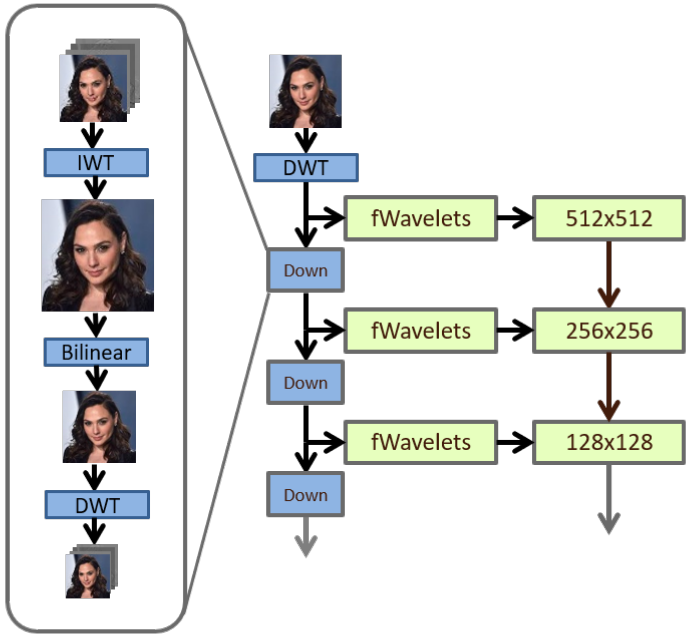
\includegraphics[width=0.5\textwidth]{imgs/Coigan/swagan_discriminator.png}
    \caption{Figura che illustra concettualmente la struttura interna del discriminatore basato sulla trasformata \textit{wavelet}.}
    \label{fig:wavelet_discriminator}
\end{figure}

Una parte importante dell'addestramento di questo discriminatore, risiede nel preprocessamento dell'input, infatti il
modello non riceve in input l'immagine generata così come è ma, riceve esclusivamente le aree relative ai difetti.
Oltre all'operazione di \textit{masking} è stata applicata una separazione dei difetti in base alla classe ottenendo così
un'immagine per ogni classe, le quali vengono poi messe in \textit{stack} per ottenere un tensore di dimensione $(n \cdot c) \times h \times w$,
dove $n$ è il numero di classi, $c$ è il numero di canali di ogni immagine, $h$ e $w$ sono rispettivamente l'altezza e la larghezza dell'immagine.
Tale tensore è poi passato in input al discriminatore, il quale restituisce un singolo valore che indica se l'immagine in input è stata generata o appartiene
alla distribuzione reale.\\
Di seguito è rappresentata l'operazione di estrazione dei difetti dall'immagine generata. 
I blocchi con sfondo arancione rappresentano dei tensori, i quali contengono in \textit{stack} le immagini al loro interno,
in particolare abbiamo nel primo blocco l'immagine base con le maschere associate alla posizione dove andranno generati i difetti,
mentre nel secondo blocco è presente l'immagine generata, e nel terzo blocco sono presenti le immagini dei difetti estratti dall'immagine generata.

\begin{figure}[H]
    \centering
    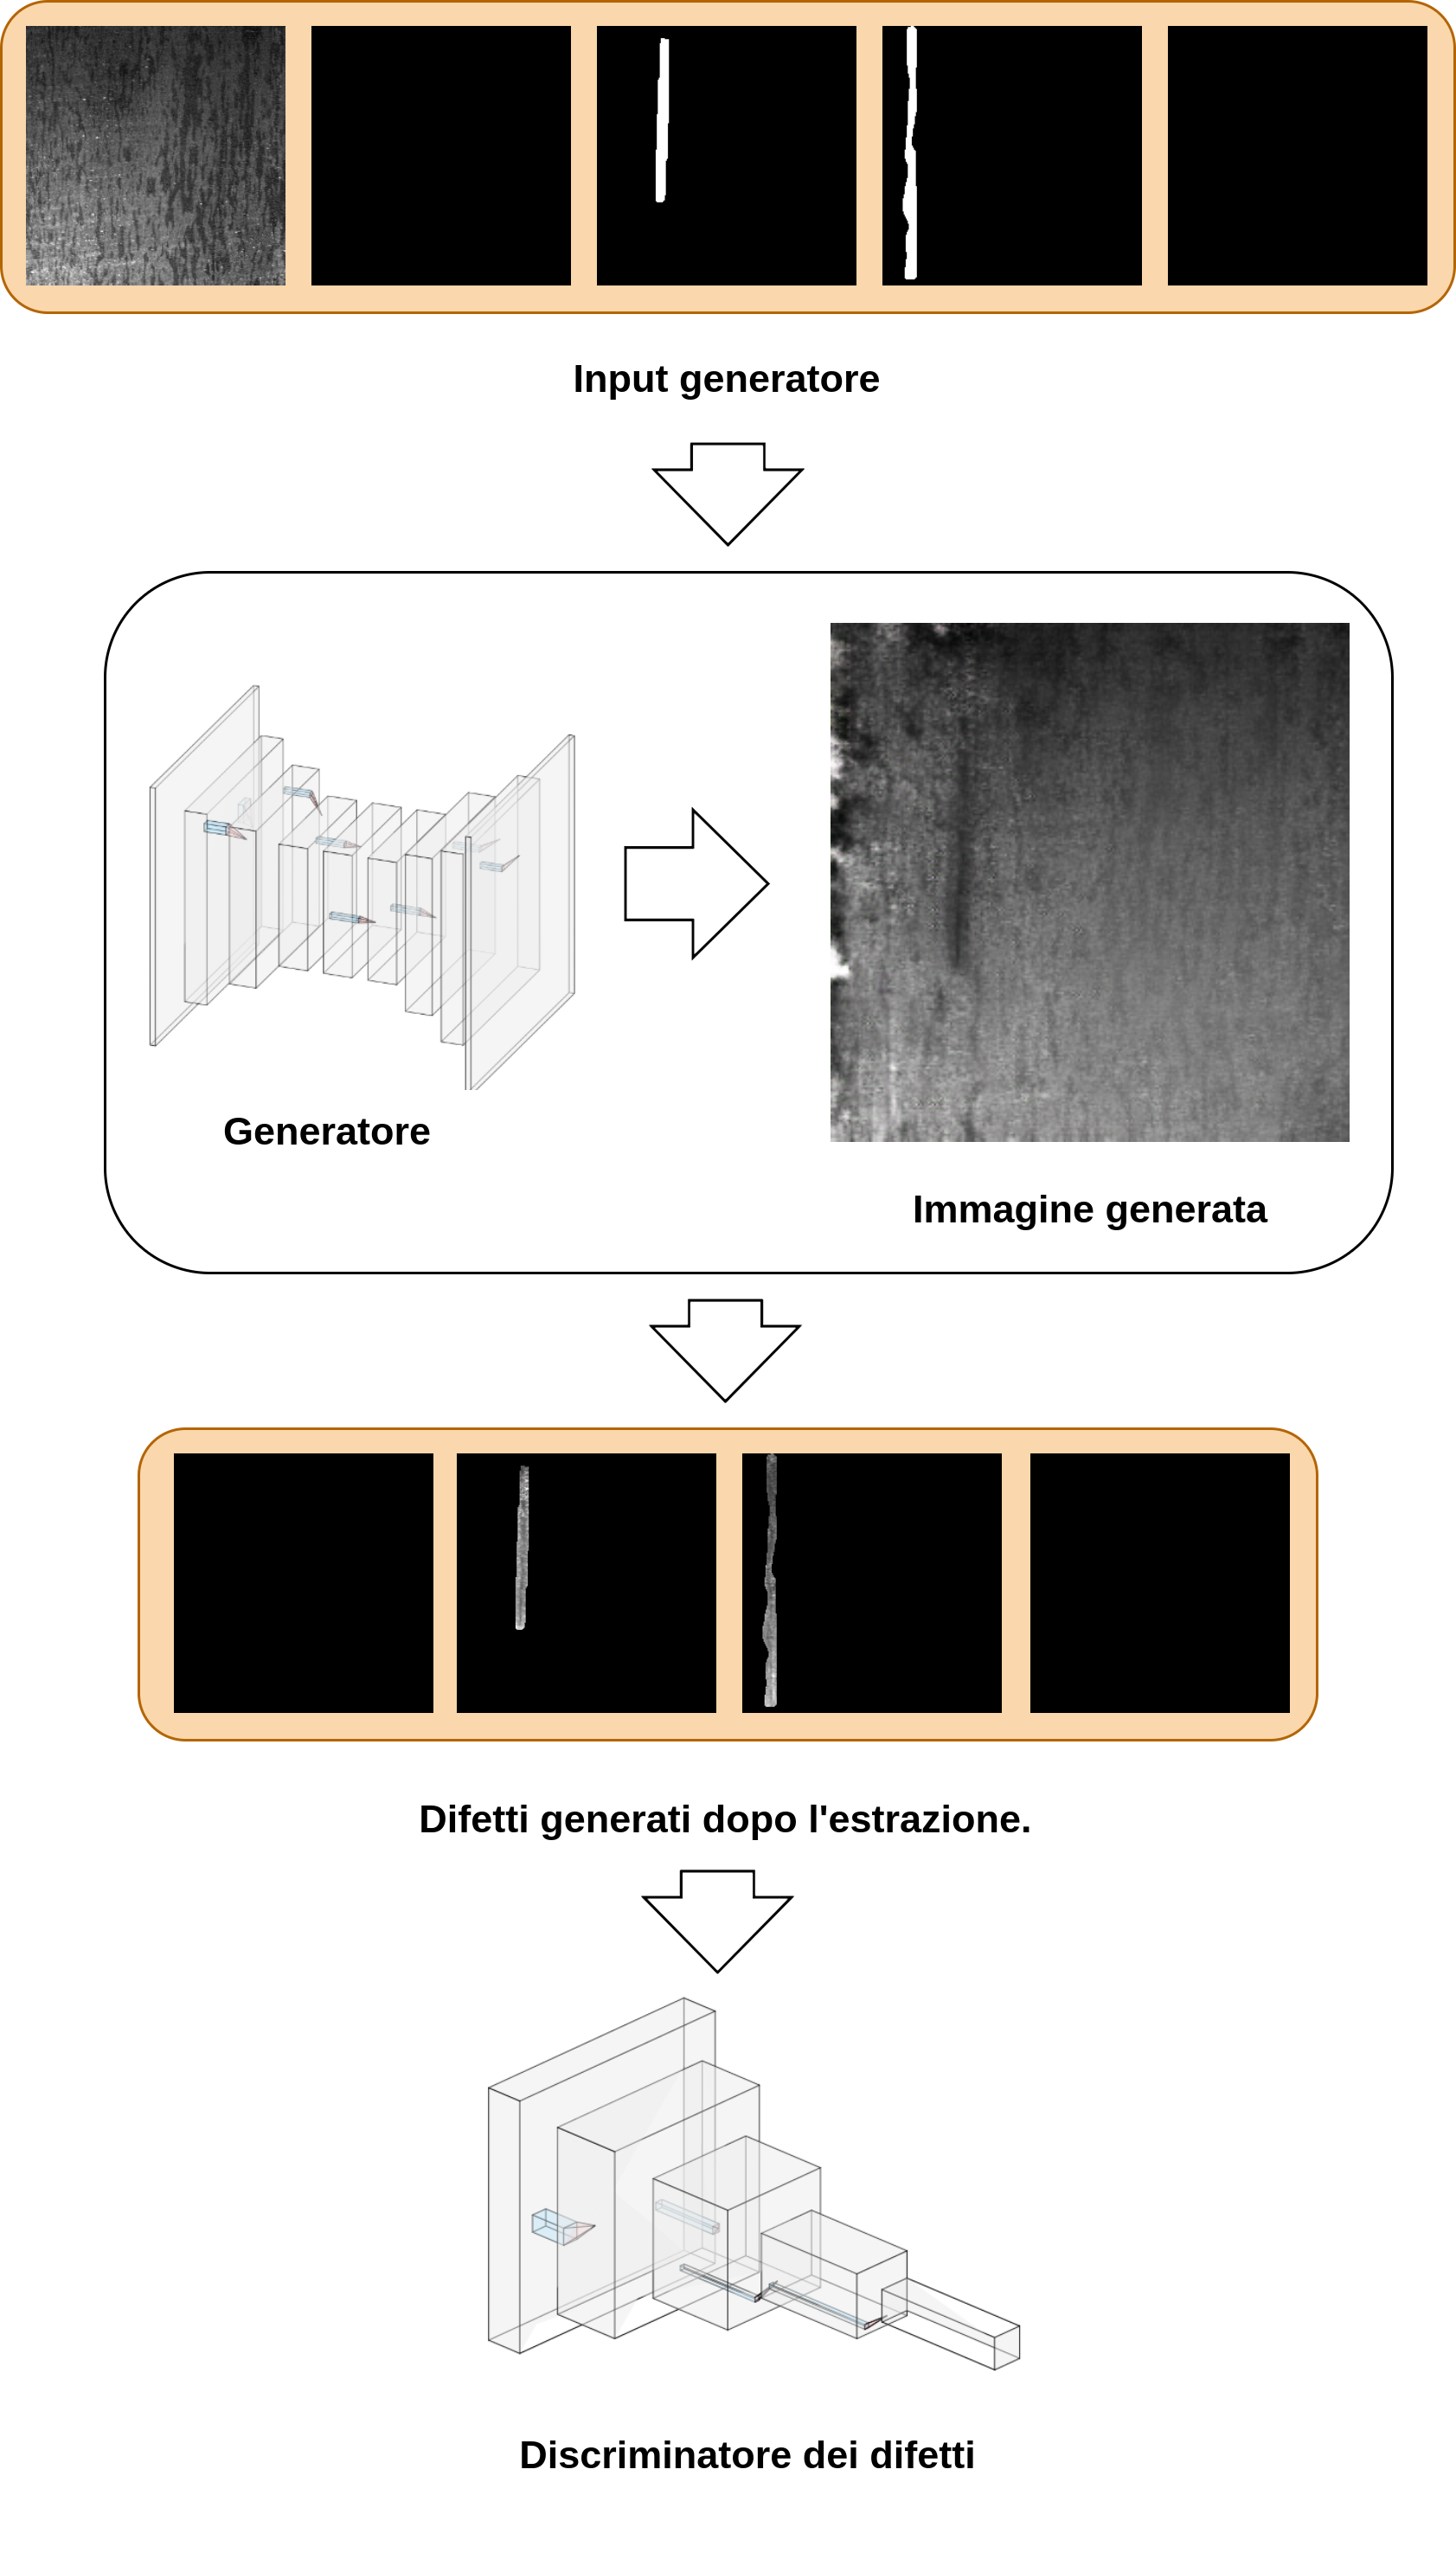
\includegraphics[width=0.55\textwidth]{imgs/Coigan/Defects_discriminator_feed.drawio.png}
    \caption{Figura che illustra concettualmente il processo di estrazione dei difetti dall'immagine generata, per l'addestramento del discriminatore.}
    \label{fig:discriminator_defects_extraction}
\end{figure}

Per l'addestramento del discriminatore è stata utilizzata la loss function proposta nella paper originale di Goodfellow et al. 
\cite{goodfellow2014generative}:
\begin{equation}
    L_{D}(G) = \mathbb{E}_{x \sim p_{data}(x)}[- \log(D(x))] + \mathbb{E}_{x \sim p_{data}(x)}[- \log(1 - D(G(x)))]
    \label{eq:discriminator_loss}
\end{equation}

Allo stesso modo anche la adversarial loss per il generatore ottenuta da questo discriminatore è quella originale
proposta nella medesima pubblicazione:
\begin{equation}
    L_{G}(D) = \mathbb{E}_{x \sim p_{data}(x)}[- \log(D(G(x)))]
    \label{eq:generator_loss}
\end{equation}
Per questo discriminatore come metodo di regolarizzazione è stata utilizzata la R1, illustrata estensivamente nella sottosezione \ref{subsubsection:r1_reg}.

\subsection{Il discriminatore di riferimento}
Il discriminatore di riferimento è il modello utilizzato per il calcolo di una loss supplementare, la quale è stata introdotta per mitigare
il problema degli artifacts sui bordi delle aree in cui è stato effettuato l'inpainting, e per cercare di risolvere un'ulteriore problema
di stacco delle tonalità di colore tra le aree rigenerate e quelle che dovrebbero essere mantenute coerenti con l'immagine base.
Nella figura \ref{fig:artifacts_example} sono mostrati alcuni esempi di immagini generate affette da artifacts e stacco delle tonalità di colore:
\begin{figure}[htbp]
    \centering
    \begin{subfigure}[b]{0.3\textwidth}
        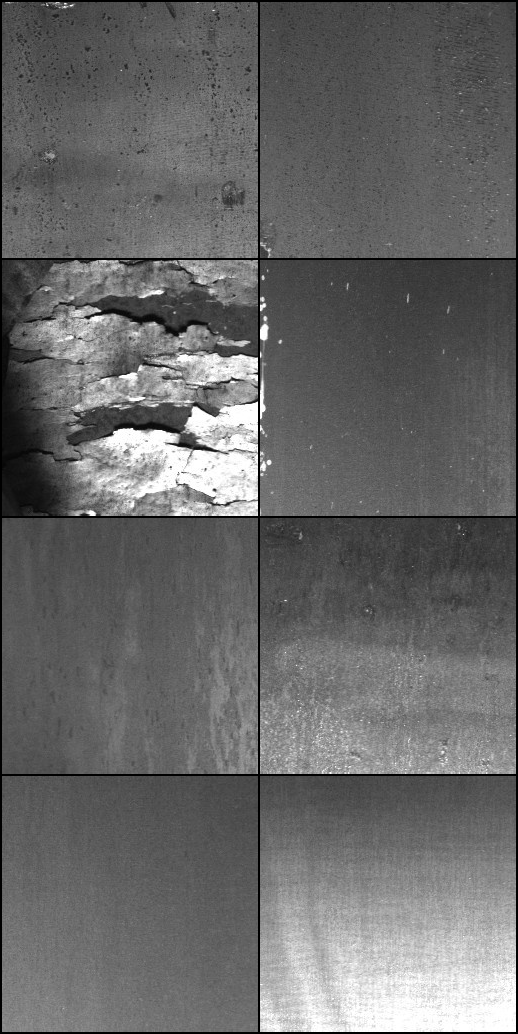
\includegraphics[width=\textwidth]{imgs/Coigan/results/artifacts/media_images_base_image_60500_ba90662d90f873ed7e4a.png}
        \caption{Immagini base.}
        \label{fig:artifacts_example_1}
    \end{subfigure}
    \hfill
    \begin{subfigure}[b]{0.3\textwidth}
        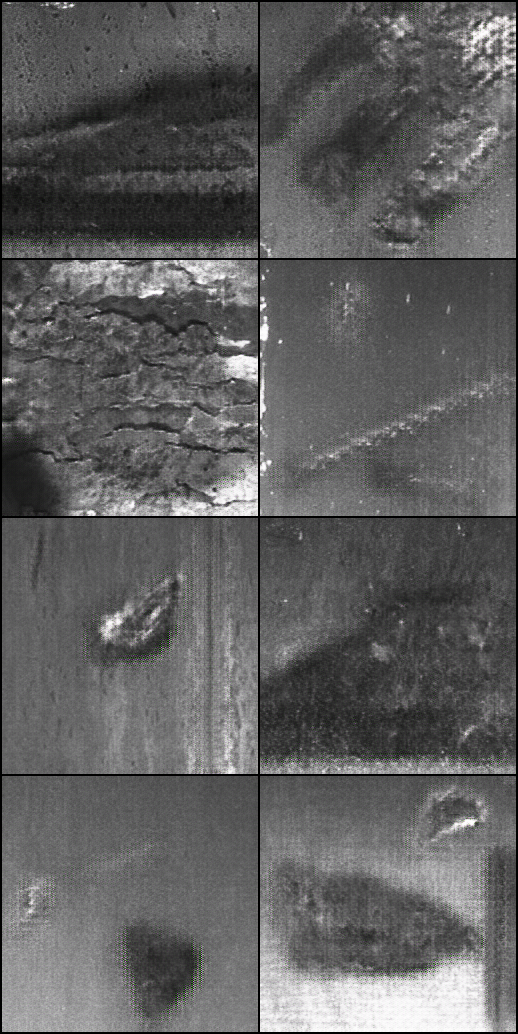
\includegraphics[width=\textwidth]{imgs/Coigan/results/artifacts/media_images_fake_image_60500_b51fd0e318bb0b991db0.png}
        \caption{Immagini generate.}
        \label{fig:artifacts_example_2}
    \end{subfigure}
    \hfill
    \begin{subfigure}[b]{0.3\textwidth}
        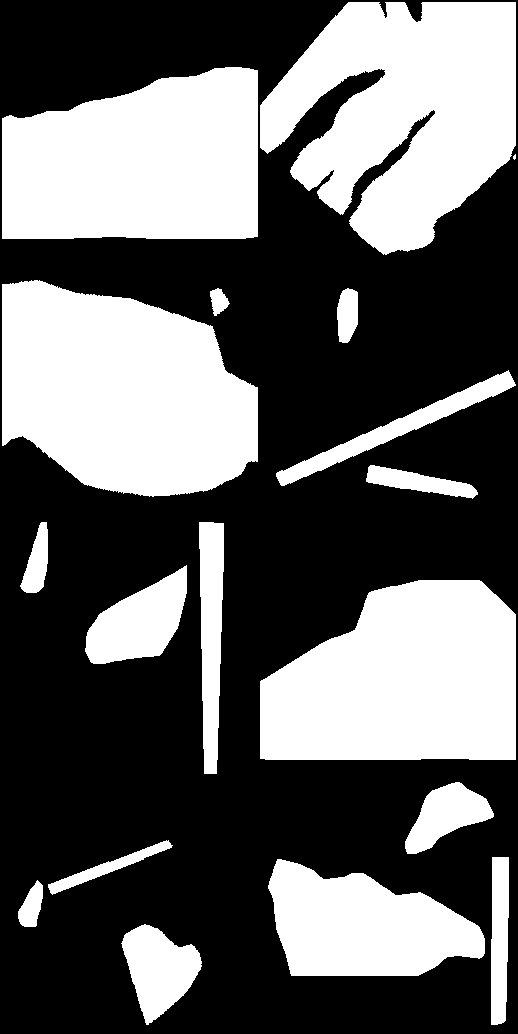
\includegraphics[width=\textwidth]{imgs/Coigan/results/artifacts/media_images_union_shapes_60500_fef7b7fd942533d3c91b.png}
        \caption{Maschere di input.}
        \label{fig:artifacts_example_3}
    \end{subfigure}
    \caption{Figura che illustra un batch di immagini generate, da una precedente versione della training pipeline, non provvista di
    \textbf{ref discriminator}, e con le loss \textbf{L1} e \textbf{Perceptual loss} che non utilizzano lo smooth della weight mask.}
    \label{fig:artifacts_example}
\end{figure}
 
Nella figura \ref{fig:good_example} invece è mostrato un batch preso da un training con una versione della training pipeline che utilizza il \textbf{ref discriminator},
e con le loss \textbf{L1} e \textbf{Perceptual loss} che applica lo smooth della weight mask ed è possibile vedere come il risultato sia molto migliorato.
Il discriminatore aggiuntivo ha introdotto però un comportamento inatteso del modello, 
il quale tende ora ad alterare maggiormente anche l'area dell'immagine che non è interessata 
dalle maschere per la generazione dei difetti, anche se generalmente non genera difetti dove non richiesto e mediamente la qualità dei risultati ottenuti
è maggiore.

\begin{figure}[htpb]
    \centering
    \begin{subfigure}[b]{0.3\textwidth}
        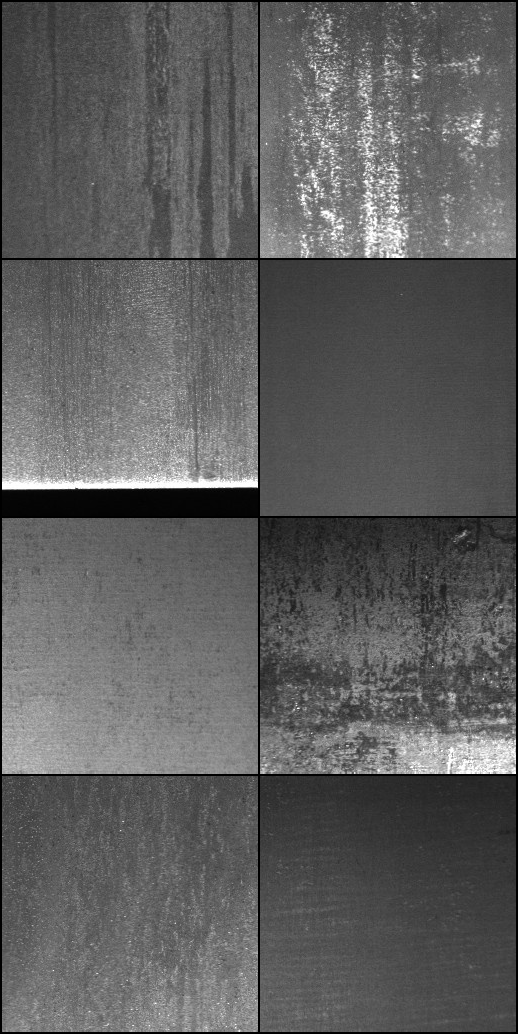
\includegraphics[width=\textwidth]{imgs/Coigan/results/buone/media_images_base_image_210000_e0ba01944dbb261374d3.png}
        \caption{Immagini base.}
        \label{fig:good_example_1}
    \end{subfigure}
    \hfill
    \begin{subfigure}[b]{0.3\textwidth}
        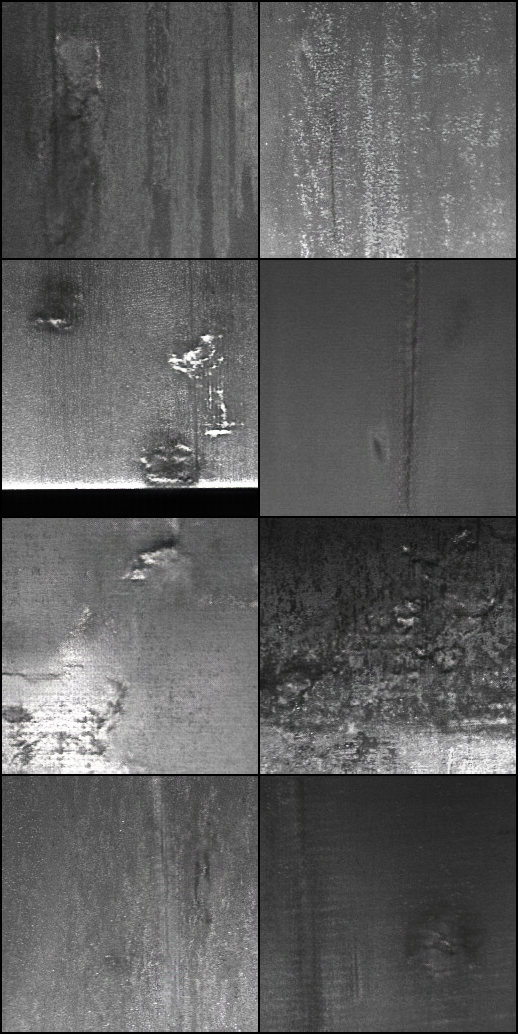
\includegraphics[width=\textwidth]{imgs/Coigan/results/buone/media_images_fake_image_210000_c481d86d1cc2f7258c70.png}
        \caption{Immagini generate.}
        \label{fig:good_example_2}
    \end{subfigure}
    \hfill
    \begin{subfigure}[b]{0.3\textwidth}
        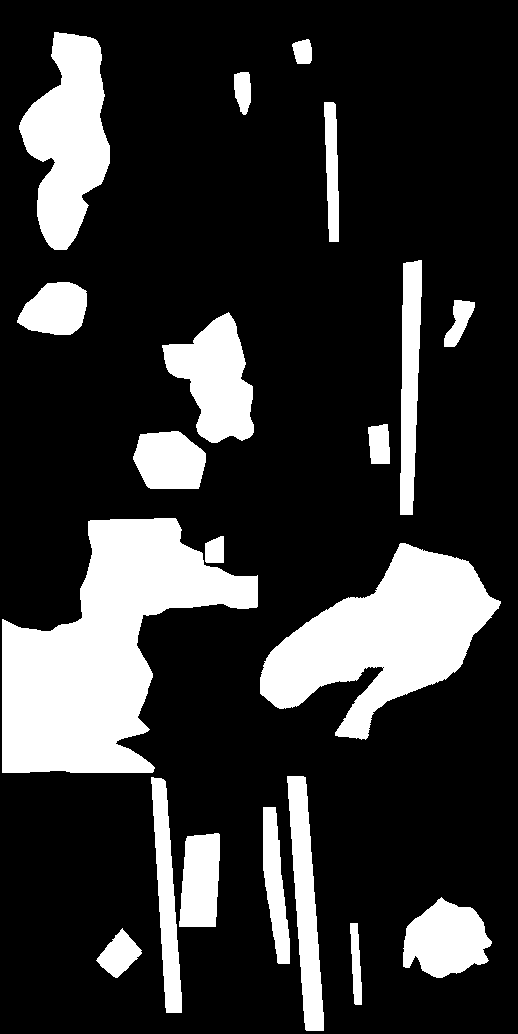
\includegraphics[width=\textwidth]{imgs/Coigan/results/buone/media_images_union_shapes_210000_00bedf5aec801c9d519d.png}
        \caption{Maschere di input.}
        \label{fig:good_example_3}
    \end{subfigure}
    \caption{Figura che illustra un batch di immagini generate, da una versione della training pipeline provvista di
    \textbf{ref discriminator}, e con le loss \textbf{L1} e \textbf{Perceptual loss} che utilizzano lo smooth della weight mask.}
    \label{fig:good_example}
\end{figure}

Anche per il discriminatore di riferimento sono state utilizzate le stesse loss e regolarizzazioni utilizzate per il discriminatore dei difetti.

\section{La valutazione del modello}
La valutazione dei risultati ottenuti da un modello di inpainting è un'operazione complessa, la quale teoricamente non può essere
effettuata in maniera accurata, in quanto per valutare la qualità di un oggetto generato non abbiamo un effettivo esempio di riferimento dalla
quale calcolare la distanza in maniera precisa.

Un primo tentativo di risolvere questo problema è stato proposto da parte di Tim Salimans et al. \cite{salimans2016improved}  nel 2016, 
i quali hanno proposto un metodo chiamato \textbf{Inception score}, il quale utilizza
un modello di \textit{image classification}, in particolare un modello \textbf{InceptionV3} pre-addestrato, per effettuare l'inferenza su un elevato numero di immagini,
(sono state utilizzate 50000 immagini generate dal modello GAN), ed utilizzare tali valori come base per stabilire la qualità del modello.
Il metodo in particolare consisteva nel valutare l'entropia delle distribuzioni delle classi predette dal modello di classificazione $p(y|x)$.
Tale metodo ha mostrato una certa somiglianza con i risultati ottenuti dagli annotatori umani attraverso lo strumento di AWS
\textbf{Mechanical Turk}. 

L'approccio di valutazione con annotatori umani ha sottolineato maggiormente la difficoltà di valutare tale tipo
di risultati, questi infatti dovevano valutare se un'immagine presentata fosse reale o generata assegnando una valutazione da 1 a 5.
Durante il processo venivano casualmente presentate immagini reali per valutare la capacità di riconoscimento degli annotatori. 
Questi ultimi hanno mostrato una certa variabilità nelle valutazioni, anche se sono stati mediamente coerenti,
inoltre è stato notato che le persone tendono a dare voti peggiori con il tempo in quanto migliorano nel riconoscere le immagini generate.

Un miglioramento dell'\textbf{Inception score} è stato proposto successivamente da Martin Heusel et al. \cite{heusel2018gans} nel 2018,
i quali hanno proposto un sistema non più basato sull'entropia della distribuzione delle classi predette,
ma bensì sulle \textit{features} estratte da un layer interno del modello di classificazione, le quali vengono confrontate tra le immagini generate e le immagini del test set.
Tale metodo è stato chiamato \textbf{Fréchet Inception Distance} (FID).

\subsection{Fréchet Inception Distance FID}
La Fréchet Inception Distance è un metodo di valutazione dei risultati ottenuti da un modello di generazione di immagini, il quale si basa sulle \textit{features} estratte
da un modello convoluzionale in uno specifico layer e non più dall'output del modello, il quale tipicamente è addestrato sul dataset \textbf{ImageNet} per la classificazione.
Come accennato la maggiore innovazione portata da questa tecnica sta nel fatto che rispetto all'\textbf{Inception score} non si basa più sull'entropia della distribuzione delle classi predette ma su una effettiva comparazione tra la distribuzione reale e quella generata che chiameremo rispettivamente $p_r$ e $p_g$.

Per rendere il calcolo della distanza non troppo complesso si fa l'assunzione che le distribuzioni $p_r$ e $p_g$ siano gaussiane multivariate, dunque
la distanza di Fréchet $d(.,.)$ tra le due distribuzioni può essere calcolata come la distanza tra le medie e le matrici di covarianza delle due distribuzioni,
ed è definita come segue:

\begin{equation}
    d(p_r, p_g) = \left \| \mu_r - \mu_g \right \|_2^2 + Tr(\Sigma_r + \Sigma_g - 2(\Sigma_r\Sigma_g)^{1/2})
\end{equation}

I due termini principali di tale equazione sono uno la distanza tra le medie delle features $\left \| \mu_r - \mu_g \right \|_2^2$, mentre l'altro
rappresenta la distanza tra le matrici di covarianza delle due distribuzioni $Tr(\Sigma_r + \Sigma_g - 2(\Sigma_r\Sigma_g)^{1/2})$.\\
I vari termini dell'equazione sono definiti di seguito:

\begin{itemize}
    \item \textbf{$\mu_r$}: media delle \textit{features} estratte dal modello InceptionV3 sul test set.
    \item \textbf{$\mu_g$}: media delle \textit{features} estratte dal modello InceptionV3 sulle immagini generate dal modello.
    \item \textbf{$\Sigma_r$}: matrice di covarianza delle \textit{features} estratte dal modello InceptionV3 sul test set.
    \item \textbf{$\Sigma_g$}: matrice di covarianza delle \textit{features} estratte dal modello InceptionV3 sulle immagini generate dal modello.
    \item \textbf{$Tr$}: traccia della matrice.
    \item \textbf{$\left \| \cdot \right \|_2$}: norma euclidea.
\end{itemize}

Anche per questo metodo è stato utilizzato il medesimo numero di immagini per generare le statistiche necessarie al calcolo della distanza, 
ovvero 50000 immagini, questa volta però sono state necessarie 50000 immagini generate dal modello e altrettante immagini del test set.

Logicamente possiamo asserire che come una valutazione data da una persona potrebbe essere estremamente soggettiva, così anche una valutazione
data da un modello convoluzionale sarà dipendente dall'addestramento del modello stesso.
Infatti si è osservato che modelli addestrati su task di classificazione ad esempio tendono a focalizzarsi su \textit{features} di basso livello, dunque textures
e colori, mentre modelli addestrati su task di segmentazione tendono a focalizzarsi su \textit{features} di alto livello, dunque forme e strutture più complesse,
tale propensione dunque si potrebbe osservare anche nel calcolo della distanza tra le distribuzioni di due insiemi di immagini, utilizzando tali
modelli.

\subsection{I risultati}
Come risultato finale del progetto si è utilizzata proprio la metrica appena presentata, la FID per valutare i risultati ottenuti dal modello.
L'effettiva procedura utilizzata è una rielaborazione dell'algoritmo originale presentato da Martin Heusel et al. \cite{heusel2018gans} nel 2018,
la quale è stata implementata con Pytorch e numpy.

Per la valutazione sono stati utilizzati i dataset di train e di test in formato tile, ovvero immagini di dimensione 256x256, e un ulteriore dataset generato
dal modello addestrato. La prima operazione è stata quella di confrontare la FID tra il set di train e il set di test, per verificare che non ci fossero
differenze significative tra le due distribuzioni, ed avere un valore di riferimento.
Tale valutazione ha portato ad un punteggio \textbf{FID: 1.0212} con 40k immagini per il training set e 40k immagini per il test set.

Il risultato ottenuto dal modello è stato più tosto alto, infatti si è ottenuto un punteggio \textbf{FID: 62.7907} confrontando 40k immagini del test set con 
40k immagini provenienti dal modello, considerando però che i difetti utilizzati per addestrare il discriminatore dei difetti erano in totale 10173
e che 2 di 4 classi avevano meno di 1000 esempi.
Tale risultato sottolinea diverse problematiche, le quali hanno portato a un risultato non ottimale, come ad esempio la presenza di \textit{artifacts} 
che se pur ridotta è ancora presente in qualche caso, e in maniera più frequente si manifestano le variazioni di colore.
Tali problemi potrebbero essere legati alla scarsità di dati, ma probabilmente con opportune modifiche alla training pipeline e al modello sarà sicuramente possibile
ottenere risultati migliori.

Facciamo a questo punto un confronto con i valori di FID ottenuti da altri modelli SOTA per vari task di generazione basati su architettura GAN:
\begin{itemize}
    \item \textbf{stylegan 2:} su FFHQ per il task di generazione di volti umani ha ottenuto un punteggio di \textbf{FID: 2.84}. Va considerato
        però che il training set consisteva di ben 70k immagini.
    \item \textbf{LaMa:} per il task di inpainting non condizionato ha ottenuto rispettivamente una \textbf{FID: 2.21} sul dataset Places con maschere di inpainting
    estese e una \textbf{FID: 7.26} sul dataset CelebA-HQ con maschere di inpainting estese.
\end{itemize}